\documentclass[twoside]{book}

% Packages required by doxygen
\usepackage{fixltx2e}
\usepackage{calc}
\usepackage{doxygen}
\usepackage[export]{adjustbox} % also loads graphicx
\usepackage{graphicx}
\usepackage[utf8]{inputenc}
\usepackage{makeidx}
\usepackage{multicol}
\usepackage{multirow}
\PassOptionsToPackage{warn}{textcomp}
\usepackage{textcomp}
\usepackage[nointegrals]{wasysym}
\usepackage[table]{xcolor}

% Font selection
\usepackage[T1]{fontenc}
\usepackage[scaled=.90]{helvet}
\usepackage{courier}
\usepackage{amssymb}
\usepackage{sectsty}
\renewcommand{\familydefault}{\sfdefault}
\allsectionsfont{%
  \fontseries{bc}\selectfont%
  \color{darkgray}%
}
\renewcommand{\DoxyLabelFont}{%
  \fontseries{bc}\selectfont%
  \color{darkgray}%
}
\newcommand{\+}{\discretionary{\mbox{\scriptsize$\hookleftarrow$}}{}{}}

% Page & text layout
\usepackage{geometry}
\geometry{%
  a4paper,%
  top=2.5cm,%
  bottom=2.5cm,%
  left=2.5cm,%
  right=2.5cm%
}
\tolerance=750
\hfuzz=15pt
\hbadness=750
\setlength{\emergencystretch}{15pt}
\setlength{\parindent}{0cm}
\setlength{\parskip}{3ex plus 2ex minus 2ex}
\makeatletter
\renewcommand{\paragraph}{%
  \@startsection{paragraph}{4}{0ex}{-1.0ex}{1.0ex}{%
    \normalfont\normalsize\bfseries\SS@parafont%
  }%
}
\renewcommand{\subparagraph}{%
  \@startsection{subparagraph}{5}{0ex}{-1.0ex}{1.0ex}{%
    \normalfont\normalsize\bfseries\SS@subparafont%
  }%
}
\makeatother

% Headers & footers
\usepackage{fancyhdr}
\pagestyle{fancyplain}
\fancyhead[LE]{\fancyplain{}{\bfseries\thepage}}
\fancyhead[CE]{\fancyplain{}{}}
\fancyhead[RE]{\fancyplain{}{\bfseries\leftmark}}
\fancyhead[LO]{\fancyplain{}{\bfseries\rightmark}}
\fancyhead[CO]{\fancyplain{}{}}
\fancyhead[RO]{\fancyplain{}{\bfseries\thepage}}
\fancyfoot[LE]{\fancyplain{}{}}
\fancyfoot[CE]{\fancyplain{}{}}
\fancyfoot[RE]{\fancyplain{}{\bfseries\scriptsize Generated by Doxygen }}
\fancyfoot[LO]{\fancyplain{}{\bfseries\scriptsize Generated by Doxygen }}
\fancyfoot[CO]{\fancyplain{}{}}
\fancyfoot[RO]{\fancyplain{}{}}
\renewcommand{\footrulewidth}{0.4pt}
\renewcommand{\chaptermark}[1]{%
  \markboth{#1}{}%
}
\renewcommand{\sectionmark}[1]{%
  \markright{\thesection\ #1}%
}

% Indices & bibliography
\usepackage{natbib}
\usepackage[titles]{tocloft}
\setcounter{tocdepth}{3}
\setcounter{secnumdepth}{5}
\makeindex

% Hyperlinks (required, but should be loaded last)
\usepackage{ifpdf}
\ifpdf
  \usepackage[pdftex,pagebackref=true]{hyperref}
\else
  \usepackage[ps2pdf,pagebackref=true]{hyperref}
\fi
\hypersetup{%
  colorlinks=true,%
  linkcolor=blue,%
  citecolor=blue,%
  unicode%
}

% Custom commands
\newcommand{\clearemptydoublepage}{%
  \newpage{\pagestyle{empty}\cleardoublepage}%
}

\usepackage{caption}
\captionsetup{labelsep=space,justification=centering,font={bf},singlelinecheck=off,skip=4pt,position=top}

%===== C O N T E N T S =====

\begin{document}

% Titlepage & ToC
\hypersetup{pageanchor=false,
             bookmarksnumbered=true,
             pdfencoding=unicode
            }
\pagenumbering{alph}
\begin{titlepage}
\vspace*{7cm}
\begin{center}%
{\Large C\+PP \\[1ex]\large 0.\+1 }\\
\vspace*{1cm}
{\large Generated by Doxygen 1.8.13}\\
\end{center}
\end{titlepage}
\clearemptydoublepage
\pagenumbering{roman}
\tableofcontents
\clearemptydoublepage
\pagenumbering{arabic}
\hypersetup{pageanchor=true}

%--- Begin generated contents ---
\chapter{Namespace Index}
\doxysection{Namespace List}
Here is a list of all documented namespaces with brief descriptions\+:\begin{DoxyCompactList}
\item\contentsline{section}{\textbf{ Les\+\_\+couches\+\_\+du\+\_\+réseau} }{\pageref{namespace_les__couches__du__r_xC3_xA9seau}}{}
\end{DoxyCompactList}

\chapter{Hierarchical Index}
\doxysection{Class Hierarchy}
This inheritance list is sorted roughly, but not completely, alphabetically\+:\begin{DoxyCompactList}
\item \contentsline{section}{Les\+\_\+couches\+\_\+du\+\_\+réseau\+::Couche}{\pageref{class_les__couches__du__r_xC3_xA9seau_1_1_couche}}{}
\begin{DoxyCompactList}
\item \contentsline{section}{Les\+\_\+couches\+\_\+du\+\_\+réseau\+::Couche\+Cachee}{\pageref{class_les__couches__du__r_xC3_xA9seau_1_1_couche_cachee}}{}
\item \contentsline{section}{Les\+\_\+couches\+\_\+du\+\_\+réseau\+::Couche\+Sorties}{\pageref{class_les__couches__du__r_xC3_xA9seau_1_1_couche_sorties}}{}
\end{DoxyCompactList}
\item \contentsline{section}{Les\+\_\+couches\+\_\+du\+\_\+réseau\+::Neurone}{\pageref{class_les__couches__du__r_xC3_xA9seau_1_1_neurone}}{}
\item \contentsline{section}{Les\+\_\+types\+\_\+de\+\_\+réseaux\+::Reseau}{\pageref{class_les__types__de__r_xC3_xA9seaux_1_1_reseau}}{}
\begin{DoxyCompactList}
\item \contentsline{section}{Les\+\_\+types\+\_\+de\+\_\+réseaux\+::Reseau\+Forwarded}{\pageref{class_les__types__de__r_xC3_xA9seaux_1_1_reseau_forwarded}}{}
\item \contentsline{section}{Les\+\_\+types\+\_\+de\+\_\+réseaux\+::Reseau\+Recurrent}{\pageref{class_les__types__de__r_xC3_xA9seaux_1_1_reseau_recurrent}}{}
\end{DoxyCompactList}
\end{DoxyCompactList}

\chapter{Class Index}
\doxysection{Class List}
Here are the classes, structs, unions and interfaces with brief descriptions\+:\begin{DoxyCompactList}
\item\contentsline{section}{\mbox{\hyperlink{class_les__couches__du__r_xC3_xA9seau_1_1_couche}{Les\+\_\+couches\+\_\+du\+\_\+réseau\+::\+Couche}} \\*Classe représentant une couche }{\pageref{class_les__couches__du__r_xC3_xA9seau_1_1_couche}}{}
\item\contentsline{section}{\mbox{\hyperlink{class_les__couches__du__r_xC3_xA9seau_1_1_couche_cachee}{Les\+\_\+couches\+\_\+du\+\_\+réseau\+::\+Couche\+Cachee}} }{\pageref{class_les__couches__du__r_xC3_xA9seau_1_1_couche_cachee}}{}
\item\contentsline{section}{\mbox{\hyperlink{class_les__couches__du__r_xC3_xA9seau_1_1_couche_sorties}{Les\+\_\+couches\+\_\+du\+\_\+réseau\+::\+Couche\+Sorties}} }{\pageref{class_les__couches__du__r_xC3_xA9seau_1_1_couche_sorties}}{}
\item\contentsline{section}{\mbox{\hyperlink{class_les__couches__du__r_xC3_xA9seau_1_1_neurone}{Les\+\_\+couches\+\_\+du\+\_\+réseau\+::\+Neurone}} \\*Classe representant un neurone }{\pageref{class_les__couches__du__r_xC3_xA9seau_1_1_neurone}}{}
\item\contentsline{section}{\mbox{\hyperlink{class_les__types__de__r_xC3_xA9seaux_1_1_reseau}{Les\+\_\+types\+\_\+de\+\_\+réseaux\+::\+Reseau}} \\*Classe representant un réseau }{\pageref{class_les__types__de__r_xC3_xA9seaux_1_1_reseau}}{}
\item\contentsline{section}{\mbox{\hyperlink{class_les__types__de__r_xC3_xA9seaux_1_1_reseau_forwarded}{Les\+\_\+types\+\_\+de\+\_\+réseaux\+::\+Reseau\+Forwarded}} }{\pageref{class_les__types__de__r_xC3_xA9seaux_1_1_reseau_forwarded}}{}
\item\contentsline{section}{\mbox{\hyperlink{class_les__types__de__r_xC3_xA9seaux_1_1_reseau_recurrent}{Les\+\_\+types\+\_\+de\+\_\+réseaux\+::\+Reseau\+Recurrent}} }{\pageref{class_les__types__de__r_xC3_xA9seaux_1_1_reseau_recurrent}}{}
\end{DoxyCompactList}

\chapter{File Index}
\section{File List}
Here is a list of all files with brief descriptions\+:\begin{DoxyCompactList}
\item\contentsline{section}{\hyperlink{_couche_8hpp}{Couche.\+hpp} \\*\hyperlink{namespace_les}{Les} propriétés d\textquotesingle{}une couche \+: son nombre de neurones ainsi que sa fonction d\textquotesingle{}activation }{\pageref{_couche_8hpp}}{}
\item\contentsline{section}{\hyperlink{_couche_cachee_8hpp}{Couche\+Cachee.\+hpp} \\*C\textquotesingle{}est un classe qui permet de créer les couches cachées du réseau, ainsi que de définir leur biais }{\pageref{_couche_cachee_8hpp}}{}
\item\contentsline{section}{\hyperlink{_couche_entrees_8hpp}{Couche\+Entrees.\+hpp} \\*La couche entrée permet de convertir nos données et d\textquotesingle{}initialiser les entrées de notre réseau }{\pageref{_couche_entrees_8hpp}}{}
\item\contentsline{section}{\hyperlink{_couche_sorties_8hpp}{Couche\+Sorties.\+hpp} \\*C\textquotesingle{}est un classe qui permet de créer la couche de sorties du réseau, ainsi que de définir leur biais }{\pageref{_couche_sorties_8hpp}}{}
\item\contentsline{section}{\hyperlink{_interface_8hpp}{Interface.\+hpp} \\*Interface Utilisateur permet de saisir divers paramètres par l\textquotesingle{}utilisateur du réseau }{\pageref{_interface_8hpp}}{}
\item\contentsline{section}{\hyperlink{_matrice_8hpp}{Matrice.\+hpp} \\*Une classe qui définit quelques opérations matricielles }{\pageref{_matrice_8hpp}}{}
\item\contentsline{section}{\hyperlink{_neurone_8hpp}{Neurone.\+hpp} \\*\hyperlink{namespace_les}{Les} propritées d\textquotesingle{}un neurone \+: son indice et so valeur }{\pageref{_neurone_8hpp}}{}
\item\contentsline{section}{\hyperlink{_reseau_8hpp}{Reseau.\+hpp} \\*\hyperlink{namespace_les}{Les} propriétés d\textquotesingle{}un réseau \+: le nombre de couches qui le compose, ses couches, et sa matrice de liaison }{\pageref{_reseau_8hpp}}{}
\item\contentsline{section}{\hyperlink{_reseau_forwarded_8hpp}{Reseau\+Forwarded.\+hpp} \\*C\textquotesingle{}est un classe qui permet de spécifier le type de réseau désiré, ici \+: type feed-\/forwarded, permet donc de préciser les arguments (forme du réseau) }{\pageref{_reseau_forwarded_8hpp}}{}
\item\contentsline{section}{\hyperlink{_reseau_recurrent_8hpp}{Reseau\+Recurrent.\+hpp} \\*C\textquotesingle{}est un classe qui permet de spécifier le type de réseau désiré, ici \+: type récurrent, permet donc de préciser les arguments (forme du réseau spécifique) }{\pageref{_reseau_recurrent_8hpp}}{}
\end{DoxyCompactList}

\chapter{Namespace Documentation}
\hypertarget{namespace_interface___saisie__des__donnees}{}\doxysection{Interface\+\_\+\+Saisie\+\_\+des\+\_\+donnees Namespace Reference}
\label{namespace_interface___saisie__des__donnees}\index{Interface\_Saisie\_des\_donnees@{Interface\_Saisie\_des\_donnees}}
\doxysubsection*{Classes}
\begin{DoxyCompactItemize}
\item 
class \mbox{\hyperlink{class_interface___saisie__des__donnees_1_1_interface}{Interface}}
\begin{DoxyCompactList}\small\item\em Classe où l\textquotesingle{}utilisateur saisit les paramètres et choix des différentes options proposées pour son futur réseau. \end{DoxyCompactList}\end{DoxyCompactItemize}


\doxysubsection{Detailed Description}
Classe permettant la saisie de données par l\textquotesingle{}utilisateur ou l\textquotesingle{}importation 
\hypertarget{namespace_les}{}\section{Les Namespace Reference}
\label{namespace_les}\index{Les@{Les}}


\subsection{Detailed Description}
couches du reseau Classe représentnant les couches du réseau 
\hypertarget{namespace_les__couches__du__reseau}{}\doxysection{Les\+\_\+couches\+\_\+du\+\_\+reseau Namespace Reference}
\label{namespace_les__couches__du__reseau}\index{Les\_couches\_du\_reseau@{Les\_couches\_du\_reseau}}
\doxysubsection*{Classes}
\begin{DoxyCompactItemize}
\item 
class \mbox{\hyperlink{class_les__couches__du__reseau_1_1_couche}{Couche}}
\begin{DoxyCompactList}\small\item\em Classe représentant une couche. \end{DoxyCompactList}\item 
class \mbox{\hyperlink{class_les__couches__du__reseau_1_1_couche_cachee}{Couche\+Cachee}}
\item 
class \mbox{\hyperlink{class_les__couches__du__reseau_1_1_couche_entrees}{Couche\+Entrees}}
\begin{DoxyCompactList}\small\item\em Classe représentant la couche d\textquotesingle{}entrée. \end{DoxyCompactList}\item 
class \mbox{\hyperlink{class_les__couches__du__reseau_1_1_couche_sorties}{Couche\+Sorties}}
\begin{DoxyCompactList}\small\item\em Classe représentant la couche de sorties. \end{DoxyCompactList}\item 
class \mbox{\hyperlink{class_les__couches__du__reseau_1_1_neurone}{Neurone}}
\begin{DoxyCompactList}\small\item\em Classe représentant un neurone. \end{DoxyCompactList}\end{DoxyCompactItemize}


\doxysubsection{Detailed Description}
Ensemble de classes représentant toutes les couches du réseau

Classe qui permet de créer des couches du réseau

Classe qui permet de créer des neurones 
\hypertarget{namespace_les__types__de__reseaux}{}\section{Les\+\_\+types\+\_\+de\+\_\+reseaux Namespace Reference}
\label{namespace_les__types__de__reseaux}\index{Les\+\_\+types\+\_\+de\+\_\+reseaux@{Les\+\_\+types\+\_\+de\+\_\+reseaux}}
\subsection*{Classes}
\begin{DoxyCompactItemize}
\item 
class \hyperlink{class_les__types__de__reseaux_1_1_matrice}{Matrice}
\item 
class \hyperlink{class_les__types__de__reseaux_1_1_reseau}{Reseau}
\begin{DoxyCompactList}\small\item\em Classe représentant un réseau. \end{DoxyCompactList}\item 
class \hyperlink{class_les__types__de__reseaux_1_1_reseau_forwarded}{Reseau\+Forwarded}
\item 
class \hyperlink{class_les__types__de__reseaux_1_1_reseau_recurrent}{Reseau\+Recurrent}
\end{DoxyCompactItemize}


\subsection{Detailed Description}
Classe pour manipuler des matrices (pour la matrice des liaisons)

Permet de créer un certain type de réseau

une classe qui permet de créer un certain type de réseau 
\chapter{Class Documentation}
\hypertarget{class_les__couches__du__reseau_1_1_couche}{}\doxysection{Les\+\_\+couches\+\_\+du\+\_\+reseau\+::Couche Class Reference}
\label{class_les__couches__du__reseau_1_1_couche}\index{Les\_couches\_du\_reseau::Couche@{Les\_couches\_du\_reseau::Couche}}


Classe représentant une couche.  




{\ttfamily \#include $<$Couche.\+hpp$>$}

Inheritance diagram for Les\+\_\+couches\+\_\+du\+\_\+reseau\+::Couche\+:\begin{figure}[H]
\begin{center}
\leavevmode
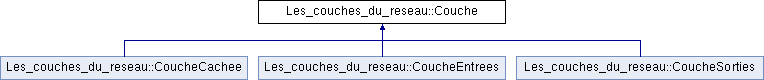
\includegraphics[height=1.458333cm]{class_les__couches__du__reseau_1_1_couche}
\end{center}
\end{figure}
\doxysubsection*{Public Member Functions}
\begin{DoxyCompactItemize}
\item 
\mbox{\hyperlink{class_les__couches__du__reseau_1_1_couche_af564932d3de118cead9fcc504e237285}{Couche}} (const int nb\+Neurones)
\begin{DoxyCompactList}\small\item\em Constructeur de la classe \mbox{\hyperlink{class_les__couches__du__reseau_1_1_couche}{Couche}}. \end{DoxyCompactList}\item 
virtual \mbox{\hyperlink{class_les__couches__du__reseau_1_1_couche_ad6b0be0bb3de03b0364a23cd64cfc052}{$\sim$\+Couche}} ()
\begin{DoxyCompactList}\small\item\em Destructeur de la classe \mbox{\hyperlink{class_les__couches__du__reseau_1_1_couche}{Couche}}. \end{DoxyCompactList}\item 
double \mbox{\hyperlink{class_les__couches__du__reseau_1_1_couche_adf4750f513cd1235edfdadb97db4f749}{pre\+Activation}} ()
\begin{DoxyCompactList}\small\item\em La fonction de pré activation \+: Méthode qui permet de faire la somme pondérée des entrées. \end{DoxyCompactList}\item 
double \mbox{\hyperlink{class_les__couches__du__reseau_1_1_couche_a9b51a1bfb515f466695e1f512da418e6}{fonc\+Activation}} (const double sum)
\begin{DoxyCompactList}\small\item\em La fonction d\textquotesingle{}activation \+: Méthode qui permet d\textquotesingle{}activer les neurones afin d\textquotesingle{}optimiser le biais et avoir le bon résultat en sortie. \end{DoxyCompactList}\end{DoxyCompactItemize}


\doxysubsection{Detailed Description}
Classe représentant une couche. 

Definition at line 18 of file Couche.\+hpp.



\doxysubsection{Constructor \& Destructor Documentation}
\mbox{\Hypertarget{class_les__couches__du__reseau_1_1_couche_af564932d3de118cead9fcc504e237285}\label{class_les__couches__du__reseau_1_1_couche_af564932d3de118cead9fcc504e237285}} 
\index{Les\_couches\_du\_reseau::Couche@{Les\_couches\_du\_reseau::Couche}!Couche@{Couche}}
\index{Couche@{Couche}!Les\_couches\_du\_reseau::Couche@{Les\_couches\_du\_reseau::Couche}}
\doxysubsubsection{\texorpdfstring{Couche()}{Couche()}}
{\footnotesize\ttfamily Les\+\_\+couches\+\_\+du\+\_\+reseau\+::\+Couche\+::\+Couche (\begin{DoxyParamCaption}\item[{const int}]{nb\+Neurones }\end{DoxyParamCaption})}



Constructeur de la classe \mbox{\hyperlink{class_les__couches__du__reseau_1_1_couche}{Couche}}. 


\begin{DoxyParams}{Parameters}
{\em nb\+Neurones} & \+: nombre fixe de neurones par couche d\textquotesingle{}où le \char`\"{}const\char`\"{} Le nombre de neurones d\textquotesingle{}une couche ne change pas une fois choisi au cours du programme \\
\hline
\end{DoxyParams}
\mbox{\Hypertarget{class_les__couches__du__reseau_1_1_couche_ad6b0be0bb3de03b0364a23cd64cfc052}\label{class_les__couches__du__reseau_1_1_couche_ad6b0be0bb3de03b0364a23cd64cfc052}} 
\index{Les\_couches\_du\_reseau::Couche@{Les\_couches\_du\_reseau::Couche}!````~Couche@{$\sim$Couche}}
\index{````~Couche@{$\sim$Couche}!Les\_couches\_du\_reseau::Couche@{Les\_couches\_du\_reseau::Couche}}
\doxysubsubsection{\texorpdfstring{$\sim$Couche()}{~Couche()}}
{\footnotesize\ttfamily virtual Les\+\_\+couches\+\_\+du\+\_\+reseau\+::\+Couche\+::$\sim$\+Couche (\begin{DoxyParamCaption}{ }\end{DoxyParamCaption})\hspace{0.3cm}{\ttfamily [virtual]}}



Destructeur de la classe \mbox{\hyperlink{class_les__couches__du__reseau_1_1_couche}{Couche}}. 



\doxysubsection{Member Function Documentation}
\mbox{\Hypertarget{class_les__couches__du__reseau_1_1_couche_a9b51a1bfb515f466695e1f512da418e6}\label{class_les__couches__du__reseau_1_1_couche_a9b51a1bfb515f466695e1f512da418e6}} 
\index{Les\_couches\_du\_reseau::Couche@{Les\_couches\_du\_reseau::Couche}!foncActivation@{foncActivation}}
\index{foncActivation@{foncActivation}!Les\_couches\_du\_reseau::Couche@{Les\_couches\_du\_reseau::Couche}}
\doxysubsubsection{\texorpdfstring{foncActivation()}{foncActivation()}}
{\footnotesize\ttfamily Les\+\_\+couches\+\_\+du\+\_\+reseau\+::\+Couche\+::fonc\+Activation (\begin{DoxyParamCaption}\item[{const double}]{sum }\end{DoxyParamCaption})}



La fonction d\textquotesingle{}activation \+: Méthode qui permet d\textquotesingle{}activer les neurones afin d\textquotesingle{}optimiser le biais et avoir le bon résultat en sortie. 

\begin{DoxyReturn}{Returns}
la valeur du neurone après l\textquotesingle{}activation 
\end{DoxyReturn}
\mbox{\Hypertarget{class_les__couches__du__reseau_1_1_couche_adf4750f513cd1235edfdadb97db4f749}\label{class_les__couches__du__reseau_1_1_couche_adf4750f513cd1235edfdadb97db4f749}} 
\index{Les\_couches\_du\_reseau::Couche@{Les\_couches\_du\_reseau::Couche}!preActivation@{preActivation}}
\index{preActivation@{preActivation}!Les\_couches\_du\_reseau::Couche@{Les\_couches\_du\_reseau::Couche}}
\doxysubsubsection{\texorpdfstring{preActivation()}{preActivation()}}
{\footnotesize\ttfamily Les\+\_\+couches\+\_\+du\+\_\+reseau\+::\+Couche\+::pre\+Activation (\begin{DoxyParamCaption}{ }\end{DoxyParamCaption})}



La fonction de pré activation \+: Méthode qui permet de faire la somme pondérée des entrées. 

\begin{DoxyReturn}{Returns}
Somme pondérée des entrées. Le résultat est passé en paramètre de la fonction d\textquotesingle{}activation 
\end{DoxyReturn}


The documentation for this class was generated from the following file\+:\begin{DoxyCompactItemize}
\item 
\mbox{\hyperlink{_couche_8hpp}{Couche.\+hpp}}\end{DoxyCompactItemize}

\hypertarget{class_les__couches__du__reseau_1_1_couche_cachee}{}\doxysection{Les\+\_\+couches\+\_\+du\+\_\+reseau\+::Couche\+Cachee Class Reference}
\label{class_les__couches__du__reseau_1_1_couche_cachee}\index{Les\_couches\_du\_reseau::CoucheCachee@{Les\_couches\_du\_reseau::CoucheCachee}}


Classe représentant la couche d\textquotesingle{}entrée.  




{\ttfamily \#include $<$Couche\+Cachee.\+hpp$>$}

Inheritance diagram for Les\+\_\+couches\+\_\+du\+\_\+reseau\+::Couche\+Cachee\+:\begin{figure}[H]
\begin{center}
\leavevmode
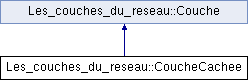
\includegraphics[height=2.000000cm]{class_les__couches__du__reseau_1_1_couche_cachee}
\end{center}
\end{figure}
\doxysubsection*{Public Member Functions}
\begin{DoxyCompactItemize}
\item 
\mbox{\hyperlink{class_les__couches__du__reseau_1_1_couche_cachee_ae721a71bbab8bf2f9cc0f8ce581844da}{Couche\+Cachee}} (const int nb\+Neurones)
\begin{DoxyCompactList}\small\item\em Constructeur de la classe \mbox{\hyperlink{class_les__couches__du__reseau_1_1_couche_cachee}{Couche\+Cachee}}. \end{DoxyCompactList}\item 
virtual \mbox{\hyperlink{class_les__couches__du__reseau_1_1_couche_cachee_a6277c5f276d60ed48d0a67768bab30d6}{$\sim$\+Couche\+Cachee}} ()
\begin{DoxyCompactList}\small\item\em Destructeur de la classe \mbox{\hyperlink{class_les__couches__du__reseau_1_1_couche_cachee}{Couche\+Cachee}}. \end{DoxyCompactList}\item 
void \mbox{\hyperlink{class_les__couches__du__reseau_1_1_couche_cachee_a87ee01348b318c64fb750e838584593d}{calcul\+Sortie}} (\mbox{\hyperlink{class_les__couches__du__reseau_1_1_couche}{Couche}} Entrees)
\begin{DoxyCompactList}\small\item\em Elle retourne la valeur en sortie de la couche après la pré-\/activation et l\textquotesingle{}activation. \end{DoxyCompactList}\end{DoxyCompactItemize}


\doxysubsection{Detailed Description}
Classe représentant la couche d\textquotesingle{}entrée. 

Definition at line 20 of file Couche\+Cachee.\+hpp.



\doxysubsection{Constructor \& Destructor Documentation}
\mbox{\Hypertarget{class_les__couches__du__reseau_1_1_couche_cachee_ae721a71bbab8bf2f9cc0f8ce581844da}\label{class_les__couches__du__reseau_1_1_couche_cachee_ae721a71bbab8bf2f9cc0f8ce581844da}} 
\index{Les\_couches\_du\_reseau::CoucheCachee@{Les\_couches\_du\_reseau::CoucheCachee}!CoucheCachee@{CoucheCachee}}
\index{CoucheCachee@{CoucheCachee}!Les\_couches\_du\_reseau::CoucheCachee@{Les\_couches\_du\_reseau::CoucheCachee}}
\doxysubsubsection{\texorpdfstring{CoucheCachee()}{CoucheCachee()}}
{\footnotesize\ttfamily Les\+\_\+couches\+\_\+du\+\_\+reseau\+::\+Couche\+Cachee\+::\+Couche\+Cachee (\begin{DoxyParamCaption}\item[{const int}]{nb\+Neurones }\end{DoxyParamCaption})}



Constructeur de la classe \mbox{\hyperlink{class_les__couches__du__reseau_1_1_couche_cachee}{Couche\+Cachee}}. 


\begin{DoxyParams}{Parameters}
{\em nb\+Neurones} & \+: nombre de neurones par couche, fixe d\textquotesingle{}où le \char`\"{}const\char`\"{} Le nombre de neurones d\textquotesingle{}une couche ne change pas au cours du programme une fois fixé ~\newline
 \\
\hline
\end{DoxyParams}
\mbox{\Hypertarget{class_les__couches__du__reseau_1_1_couche_cachee_a6277c5f276d60ed48d0a67768bab30d6}\label{class_les__couches__du__reseau_1_1_couche_cachee_a6277c5f276d60ed48d0a67768bab30d6}} 
\index{Les\_couches\_du\_reseau::CoucheCachee@{Les\_couches\_du\_reseau::CoucheCachee}!````~CoucheCachee@{$\sim$CoucheCachee}}
\index{````~CoucheCachee@{$\sim$CoucheCachee}!Les\_couches\_du\_reseau::CoucheCachee@{Les\_couches\_du\_reseau::CoucheCachee}}
\doxysubsubsection{\texorpdfstring{$\sim$CoucheCachee()}{~CoucheCachee()}}
{\footnotesize\ttfamily virtual Les\+\_\+couches\+\_\+du\+\_\+reseau\+::\+Couche\+Cachee\+::$\sim$\+Couche\+Cachee (\begin{DoxyParamCaption}{ }\end{DoxyParamCaption})\hspace{0.3cm}{\ttfamily [virtual]}}



Destructeur de la classe \mbox{\hyperlink{class_les__couches__du__reseau_1_1_couche_cachee}{Couche\+Cachee}}. 



\doxysubsection{Member Function Documentation}
\mbox{\Hypertarget{class_les__couches__du__reseau_1_1_couche_cachee_a87ee01348b318c64fb750e838584593d}\label{class_les__couches__du__reseau_1_1_couche_cachee_a87ee01348b318c64fb750e838584593d}} 
\index{Les\_couches\_du\_reseau::CoucheCachee@{Les\_couches\_du\_reseau::CoucheCachee}!calculSortie@{calculSortie}}
\index{calculSortie@{calculSortie}!Les\_couches\_du\_reseau::CoucheCachee@{Les\_couches\_du\_reseau::CoucheCachee}}
\doxysubsubsection{\texorpdfstring{calculSortie()}{calculSortie()}}
{\footnotesize\ttfamily Les\+\_\+couches\+\_\+du\+\_\+reseau\+::\+Couche\+Cachee\+::calcul\+Sortie (\begin{DoxyParamCaption}\item[{\mbox{\hyperlink{class_les__couches__du__reseau_1_1_couche}{Couche}}}]{Entrees }\end{DoxyParamCaption})}



Elle retourne la valeur en sortie de la couche après la pré-\/activation et l\textquotesingle{}activation. 


\begin{DoxyParams}{Parameters}
{\em La} & couche en entrée \\
\hline
\end{DoxyParams}
\begin{DoxyReturn}{Returns}
la valeur en sortie d\textquotesingle{}une couche 
\end{DoxyReturn}


The documentation for this class was generated from the following file\+:\begin{DoxyCompactItemize}
\item 
\mbox{\hyperlink{_couche_cachee_8hpp}{Couche\+Cachee.\+hpp}}\end{DoxyCompactItemize}

\hypertarget{class_couche_cach_xC3_xA9e}{}\section{Couche\+Cachée Class Reference}
\label{class_couche_cach_xC3_xA9e}\index{Couche\+Cachée@{Couche\+Cachée}}


Classe representant une couche.  




{\ttfamily \#include $<$Couche\+Cachee.\+hpp$>$}



\subsection{Detailed Description}
Classe representant une couche. 

The documentation for this class was generated from the following file\+:\begin{DoxyCompactItemize}
\item 
\hyperlink{_couche_cachee_8hpp}{Couche\+Cachee.\+hpp}\end{DoxyCompactItemize}

\hypertarget{class_les__couches__du__reseau_1_1_couche_entrees}{}\section{Les\+\_\+couches\+\_\+du\+\_\+reseau\+:\+:Couche\+Entrees Class Reference}
\label{class_les__couches__du__reseau_1_1_couche_entrees}\index{Les\+\_\+couches\+\_\+du\+\_\+reseau\+::\+Couche\+Entrees@{Les\+\_\+couches\+\_\+du\+\_\+reseau\+::\+Couche\+Entrees}}


Classe representant une couche.  




{\ttfamily \#include $<$Couche\+Entrees.\+hpp$>$}



Inheritance diagram for Les\+\_\+couches\+\_\+du\+\_\+reseau\+:\+:Couche\+Entrees\+:\nopagebreak
\begin{figure}[H]
\begin{center}
\leavevmode
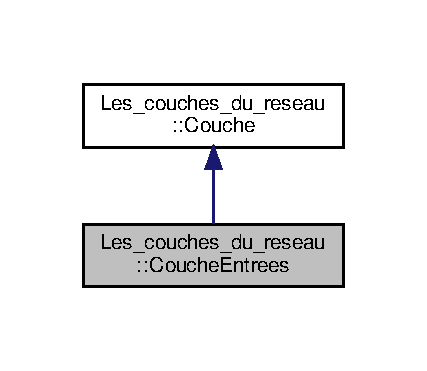
\includegraphics[width=205pt]{class_les__couches__du__reseau_1_1_couche_entrees__inherit__graph}
\end{center}
\end{figure}


Collaboration diagram for Les\+\_\+couches\+\_\+du\+\_\+reseau\+:\+:Couche\+Entrees\+:\nopagebreak
\begin{figure}[H]
\begin{center}
\leavevmode
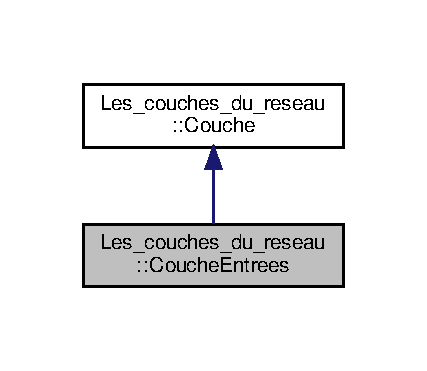
\includegraphics[width=205pt]{class_les__couches__du__reseau_1_1_couche_entrees__coll__graph}
\end{center}
\end{figure}
\subsection*{Public Member Functions}
\begin{DoxyCompactItemize}
\item 
\hyperlink{class_les__couches__du__reseau_1_1_couche_entrees_a880aff72f6d9dfa97a8f38aed085e28b}{Couche\+Entrees} (const int nb\+Neurones)
\begin{DoxyCompactList}\small\item\em Constructeur de la classe \hyperlink{class_les__couches__du__reseau_1_1_couche_entrees}{Couche\+Entrees}. \end{DoxyCompactList}\item 
virtual \hyperlink{class_les__couches__du__reseau_1_1_couche_entrees_ac672754ca6746650c139d3b22d5c611c}{$\sim$\+Couche\+Entrees} ()
\begin{DoxyCompactList}\small\item\em Destructeur de la classe \hyperlink{class_les__couches__du__reseau_1_1_couche_entrees}{Couche\+Entrees}. \end{DoxyCompactList}\item 
void \hyperlink{class_les__couches__du__reseau_1_1_couche_entrees_a52ed50cfc77b6aa116e1966faa349759}{construction\+Sortie} ()
\begin{DoxyCompactList}\small\item\em initialise les données \end{DoxyCompactList}\end{DoxyCompactItemize}


\subsection{Detailed Description}
Classe representant une couche. 

C\textquotesingle{}est la classe qui génère les couches du réseau 

\subsection{Constructor \& Destructor Documentation}
\mbox{\Hypertarget{class_les__couches__du__reseau_1_1_couche_entrees_a880aff72f6d9dfa97a8f38aed085e28b}\label{class_les__couches__du__reseau_1_1_couche_entrees_a880aff72f6d9dfa97a8f38aed085e28b}} 
\index{Les\+\_\+couches\+\_\+du\+\_\+reseau\+::\+Couche\+Entrees@{Les\+\_\+couches\+\_\+du\+\_\+reseau\+::\+Couche\+Entrees}!Couche\+Entrees@{Couche\+Entrees}}
\index{Couche\+Entrees@{Couche\+Entrees}!Les\+\_\+couches\+\_\+du\+\_\+reseau\+::\+Couche\+Entrees@{Les\+\_\+couches\+\_\+du\+\_\+reseau\+::\+Couche\+Entrees}}
\subsubsection{\texorpdfstring{Couche\+Entrees()}{CoucheEntrees()}}
{\footnotesize\ttfamily Les\+\_\+couches\+\_\+du\+\_\+reseau\+::\+Couche\+Entrees\+::\+Couche\+Entrees (\begin{DoxyParamCaption}\item[{const int}]{nb\+Neurones }\end{DoxyParamCaption})}



Constructeur de la classe \hyperlink{class_les__couches__du__reseau_1_1_couche_entrees}{Couche\+Entrees}. 


\begin{DoxyParams}{Parameters}
{\em nb\+Neurones} & \+: nombre de neurones par couche, fixe d\textquotesingle{}où le \char`\"{}const\char`\"{}nb de Neurones d\textquotesingle{}une couche ne change pas une fois choisi au cours du programme \\
\hline
\end{DoxyParams}
\mbox{\Hypertarget{class_les__couches__du__reseau_1_1_couche_entrees_ac672754ca6746650c139d3b22d5c611c}\label{class_les__couches__du__reseau_1_1_couche_entrees_ac672754ca6746650c139d3b22d5c611c}} 
\index{Les\+\_\+couches\+\_\+du\+\_\+reseau\+::\+Couche\+Entrees@{Les\+\_\+couches\+\_\+du\+\_\+reseau\+::\+Couche\+Entrees}!````~Couche\+Entrees@{$\sim$\+Couche\+Entrees}}
\index{````~Couche\+Entrees@{$\sim$\+Couche\+Entrees}!Les\+\_\+couches\+\_\+du\+\_\+reseau\+::\+Couche\+Entrees@{Les\+\_\+couches\+\_\+du\+\_\+reseau\+::\+Couche\+Entrees}}
\subsubsection{\texorpdfstring{$\sim$\+Couche\+Entrees()}{~CoucheEntrees()}}
{\footnotesize\ttfamily virtual Les\+\_\+couches\+\_\+du\+\_\+reseau\+::\+Couche\+Entrees\+::$\sim$\+Couche\+Entrees (\begin{DoxyParamCaption}{ }\end{DoxyParamCaption})\hspace{0.3cm}{\ttfamily [virtual]}}



Destructeur de la classe \hyperlink{class_les__couches__du__reseau_1_1_couche_entrees}{Couche\+Entrees}. 



\subsection{Member Function Documentation}
\mbox{\Hypertarget{class_les__couches__du__reseau_1_1_couche_entrees_a52ed50cfc77b6aa116e1966faa349759}\label{class_les__couches__du__reseau_1_1_couche_entrees_a52ed50cfc77b6aa116e1966faa349759}} 
\index{Les\+\_\+couches\+\_\+du\+\_\+reseau\+::\+Couche\+Entrees@{Les\+\_\+couches\+\_\+du\+\_\+reseau\+::\+Couche\+Entrees}!construction\+Sortie@{construction\+Sortie}}
\index{construction\+Sortie@{construction\+Sortie}!Les\+\_\+couches\+\_\+du\+\_\+reseau\+::\+Couche\+Entrees@{Les\+\_\+couches\+\_\+du\+\_\+reseau\+::\+Couche\+Entrees}}
\subsubsection{\texorpdfstring{construction\+Sortie()}{constructionSortie()}}
{\footnotesize\ttfamily Les\+\_\+couches\+\_\+du\+\_\+reseau\+::\+Couche\+Entrees\+::construction\+Sortie (\begin{DoxyParamCaption}{ }\end{DoxyParamCaption})}



initialise les données 

\begin{DoxyReturn}{Returns}
\hyperlink{namespace_les}{Les} entrées du réseau 
\end{DoxyReturn}


The documentation for this class was generated from the following file\+:\begin{DoxyCompactItemize}
\item 
\hyperlink{_couche_entrees_8hpp}{Couche\+Entrees.\+hpp}\end{DoxyCompactItemize}

\hypertarget{class_les__couches__du__reseau_1_1_couche_sorties}{}\doxysection{Les\+\_\+couches\+\_\+du\+\_\+reseau\+::Couche\+Sorties Class Reference}
\label{class_les__couches__du__reseau_1_1_couche_sorties}\index{Les\_couches\_du\_reseau::CoucheSorties@{Les\_couches\_du\_reseau::CoucheSorties}}


Classe représentant la couche de sorties.  




{\ttfamily \#include $<$Couche\+Sorties.\+hpp$>$}

Inheritance diagram for Les\+\_\+couches\+\_\+du\+\_\+reseau\+::Couche\+Sorties\+:\begin{figure}[H]
\begin{center}
\leavevmode
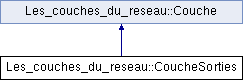
\includegraphics[height=2.000000cm]{class_les__couches__du__reseau_1_1_couche_sorties}
\end{center}
\end{figure}
\doxysubsection*{Public Member Functions}
\begin{DoxyCompactItemize}
\item 
\mbox{\hyperlink{class_les__couches__du__reseau_1_1_couche_sorties_a24c107da84b3406fedfe0071750a054b}{Couche\+Sorties}} ()
\begin{DoxyCompactList}\small\item\em Constructeur de la classe \mbox{\hyperlink{class_les__couches__du__reseau_1_1_couche_sorties}{Couche\+Sorties}}. \end{DoxyCompactList}\item 
virtual \mbox{\hyperlink{class_les__couches__du__reseau_1_1_couche_sorties_a0f1a57f483686a6d14582f40aef38299}{$\sim$\+Couche\+Sorties}} ()
\begin{DoxyCompactList}\small\item\em Destructeur de la classe \mbox{\hyperlink{class_les__couches__du__reseau_1_1_couche_sorties}{Couche\+Sorties}}. \end{DoxyCompactList}\item 
void \mbox{\hyperlink{class_les__couches__du__reseau_1_1_couche_sorties_a5d206488b6fed1e3e8ca6b06ae04688d}{construction\+Sorties}} ()
\begin{DoxyCompactList}\small\item\em La fonction calcule la sortie du réseau. \end{DoxyCompactList}\end{DoxyCompactItemize}


\doxysubsection{Detailed Description}
Classe représentant la couche de sorties. 

Definition at line 21 of file Couche\+Sorties.\+hpp.



\doxysubsection{Constructor \& Destructor Documentation}
\mbox{\Hypertarget{class_les__couches__du__reseau_1_1_couche_sorties_a24c107da84b3406fedfe0071750a054b}\label{class_les__couches__du__reseau_1_1_couche_sorties_a24c107da84b3406fedfe0071750a054b}} 
\index{Les\_couches\_du\_reseau::CoucheSorties@{Les\_couches\_du\_reseau::CoucheSorties}!CoucheSorties@{CoucheSorties}}
\index{CoucheSorties@{CoucheSorties}!Les\_couches\_du\_reseau::CoucheSorties@{Les\_couches\_du\_reseau::CoucheSorties}}
\doxysubsubsection{\texorpdfstring{CoucheSorties()}{CoucheSorties()}}
{\footnotesize\ttfamily Les\+\_\+couches\+\_\+du\+\_\+reseau\+::\+Couche\+Sorties\+::\+Couche\+Sorties (\begin{DoxyParamCaption}{ }\end{DoxyParamCaption})}



Constructeur de la classe \mbox{\hyperlink{class_les__couches__du__reseau_1_1_couche_sorties}{Couche\+Sorties}}. 

nb de Neurones d\textquotesingle{}une couche ne change pas une fois choisi au cours du programme \mbox{\Hypertarget{class_les__couches__du__reseau_1_1_couche_sorties_a0f1a57f483686a6d14582f40aef38299}\label{class_les__couches__du__reseau_1_1_couche_sorties_a0f1a57f483686a6d14582f40aef38299}} 
\index{Les\_couches\_du\_reseau::CoucheSorties@{Les\_couches\_du\_reseau::CoucheSorties}!````~CoucheSorties@{$\sim$CoucheSorties}}
\index{````~CoucheSorties@{$\sim$CoucheSorties}!Les\_couches\_du\_reseau::CoucheSorties@{Les\_couches\_du\_reseau::CoucheSorties}}
\doxysubsubsection{\texorpdfstring{$\sim$CoucheSorties()}{~CoucheSorties()}}
{\footnotesize\ttfamily virtual Les\+\_\+couches\+\_\+du\+\_\+reseau\+::\+Couche\+Sorties\+::$\sim$\+Couche\+Sorties (\begin{DoxyParamCaption}{ }\end{DoxyParamCaption})\hspace{0.3cm}{\ttfamily [virtual]}}



Destructeur de la classe \mbox{\hyperlink{class_les__couches__du__reseau_1_1_couche_sorties}{Couche\+Sorties}}. 



\doxysubsection{Member Function Documentation}
\mbox{\Hypertarget{class_les__couches__du__reseau_1_1_couche_sorties_a5d206488b6fed1e3e8ca6b06ae04688d}\label{class_les__couches__du__reseau_1_1_couche_sorties_a5d206488b6fed1e3e8ca6b06ae04688d}} 
\index{Les\_couches\_du\_reseau::CoucheSorties@{Les\_couches\_du\_reseau::CoucheSorties}!constructionSorties@{constructionSorties}}
\index{constructionSorties@{constructionSorties}!Les\_couches\_du\_reseau::CoucheSorties@{Les\_couches\_du\_reseau::CoucheSorties}}
\doxysubsubsection{\texorpdfstring{constructionSorties()}{constructionSorties()}}
{\footnotesize\ttfamily Les\+\_\+couches\+\_\+du\+\_\+reseau\+::\+Couche\+Sorties\+::construction\+Sorties (\begin{DoxyParamCaption}{ }\end{DoxyParamCaption})}



La fonction calcule la sortie du réseau. 

\begin{DoxyReturn}{Returns}
résultat du reseau 
\end{DoxyReturn}


The documentation for this class was generated from the following file\+:\begin{DoxyCompactItemize}
\item 
\mbox{\hyperlink{_couche_sorties_8hpp}{Couche\+Sorties.\+hpp}}\end{DoxyCompactItemize}

\hypertarget{class_interface___saisie__des__donnees_1_1_interface}{}\doxysection{Interface\+\_\+\+Saisie\+\_\+des\+\_\+donnees\+::Interface Class Reference}
\label{class_interface___saisie__des__donnees_1_1_interface}\index{Interface\_Saisie\_des\_donnees::Interface@{Interface\_Saisie\_des\_donnees::Interface}}


Classe où l\textquotesingle{}utilisateur saisit les paramètres et choix des différentes options proposées pour son futur réseau.  




{\ttfamily \#include $<$Interface.\+hpp$>$}

\doxysubsection*{Public Member Functions}
\begin{DoxyCompactItemize}
\item 
\mbox{\hyperlink{class_interface___saisie__des__donnees_1_1_interface_a72c791f0d80f2f93845f61ad679f11ec}{Interface}} ()
\begin{DoxyCompactList}\small\item\em Constructeur. \end{DoxyCompactList}\item 
double $\ast$ \mbox{\hyperlink{class_interface___saisie__des__donnees_1_1_interface_a5cd79d6131ec57d8e32f74772ee553b2}{lecture\+Fichier}} (char nom\+Fic\mbox{[}100\mbox{]})
\begin{DoxyCompactList}\small\item\em Importation des paramètres par un fichier de données et convertion en liste et lecture des paramètre du futur réseau de neurone dans un fichier ~\newline
 \end{DoxyCompactList}\item 
double $\ast$ \mbox{\hyperlink{class_interface___saisie__des__donnees_1_1_interface_a290c3761a31998630c1245c8a4b7ef5a}{lecture\+Param}} ()
\begin{DoxyCompactList}\small\item\em Importation des paramètres par saisie de l\textquotesingle{}utilisateur dans le terminal Lecture des paramètres du futur réseau de neurone dans le terminal. \end{DoxyCompactList}\end{DoxyCompactItemize}


\doxysubsection{Detailed Description}
Classe où l\textquotesingle{}utilisateur saisit les paramètres et choix des différentes options proposées pour son futur réseau. 

Definition at line 17 of file Interface.\+hpp.



\doxysubsection{Constructor \& Destructor Documentation}
\mbox{\Hypertarget{class_interface___saisie__des__donnees_1_1_interface_a72c791f0d80f2f93845f61ad679f11ec}\label{class_interface___saisie__des__donnees_1_1_interface_a72c791f0d80f2f93845f61ad679f11ec}} 
\index{Interface\_Saisie\_des\_donnees::Interface@{Interface\_Saisie\_des\_donnees::Interface}!Interface@{Interface}}
\index{Interface@{Interface}!Interface\_Saisie\_des\_donnees::Interface@{Interface\_Saisie\_des\_donnees::Interface}}
\doxysubsubsection{\texorpdfstring{Interface()}{Interface()}}
{\footnotesize\ttfamily Interface\+\_\+\+Saisie\+\_\+des\+\_\+donnees\+::\+Interface\+::\+Interface (\begin{DoxyParamCaption}{ }\end{DoxyParamCaption})}



Constructeur. 

Constructeur de l\textquotesingle{}interface 

\doxysubsection{Member Function Documentation}
\mbox{\Hypertarget{class_interface___saisie__des__donnees_1_1_interface_a5cd79d6131ec57d8e32f74772ee553b2}\label{class_interface___saisie__des__donnees_1_1_interface_a5cd79d6131ec57d8e32f74772ee553b2}} 
\index{Interface\_Saisie\_des\_donnees::Interface@{Interface\_Saisie\_des\_donnees::Interface}!lectureFichier@{lectureFichier}}
\index{lectureFichier@{lectureFichier}!Interface\_Saisie\_des\_donnees::Interface@{Interface\_Saisie\_des\_donnees::Interface}}
\doxysubsubsection{\texorpdfstring{lectureFichier()}{lectureFichier()}}
{\footnotesize\ttfamily Interface\+\_\+\+Saisie\+\_\+des\+\_\+donnees\+::\+Interface\+::lecture\+Fichier (\begin{DoxyParamCaption}\item[{char}]{nom\+Fic\mbox{[}100\mbox{]} }\end{DoxyParamCaption})}



Importation des paramètres par un fichier de données et convertion en liste et lecture des paramètre du futur réseau de neurone dans un fichier ~\newline
 

\begin{DoxyReturn}{Returns}
une liste des paramètres du futur réseau de neurone 
\end{DoxyReturn}
\mbox{\Hypertarget{class_interface___saisie__des__donnees_1_1_interface_a290c3761a31998630c1245c8a4b7ef5a}\label{class_interface___saisie__des__donnees_1_1_interface_a290c3761a31998630c1245c8a4b7ef5a}} 
\index{Interface\_Saisie\_des\_donnees::Interface@{Interface\_Saisie\_des\_donnees::Interface}!lectureParam@{lectureParam}}
\index{lectureParam@{lectureParam}!Interface\_Saisie\_des\_donnees::Interface@{Interface\_Saisie\_des\_donnees::Interface}}
\doxysubsubsection{\texorpdfstring{lectureParam()}{lectureParam()}}
{\footnotesize\ttfamily Interface\+\_\+\+Saisie\+\_\+des\+\_\+donnees\+::\+Interface\+::lecture\+Param (\begin{DoxyParamCaption}{ }\end{DoxyParamCaption})}



Importation des paramètres par saisie de l\textquotesingle{}utilisateur dans le terminal Lecture des paramètres du futur réseau de neurone dans le terminal. 

\begin{DoxyReturn}{Returns}
une liste des paramètres du futur réseau de neurone 
\end{DoxyReturn}


The documentation for this class was generated from the following file\+:\begin{DoxyCompactItemize}
\item 
\mbox{\hyperlink{_interface_8hpp}{Interface.\+hpp}}\end{DoxyCompactItemize}

\hypertarget{class_les__types__de__reseaux_1_1_matrice}{}\section{Les\+\_\+types\+\_\+de\+\_\+reseaux\+:\+:Matrice Class Reference}
\label{class_les__types__de__reseaux_1_1_matrice}\index{Les\+\_\+types\+\_\+de\+\_\+reseaux\+::\+Matrice@{Les\+\_\+types\+\_\+de\+\_\+reseaux\+::\+Matrice}}


{\ttfamily \#include $<$Matrice.\+hpp$>$}

\subsection*{Public Member Functions}
\begin{DoxyCompactItemize}
\item 
\hyperlink{class_les__types__de__reseaux_1_1_matrice_a7a0b8038807072d949544f0dc2a9fcb2}{Matrice} (const int nb\+Lignes, const int nb\+Colonnes)
\begin{DoxyCompactList}\small\item\em Constructeur \hyperlink{class_les__types__de__reseaux_1_1_matrice}{Matrice}. \end{DoxyCompactList}\item 
virtual \hyperlink{class_les__types__de__reseaux_1_1_matrice_a2ff1d0b7e835d4b3c4b8f266083e67c6}{$\sim$\+Matrice} ()
\begin{DoxyCompactList}\small\item\em Destructeur \hyperlink{class_les__types__de__reseaux_1_1_matrice}{Matrice}. \end{DoxyCompactList}\item 
void \hyperlink{class_les__types__de__reseaux_1_1_matrice_ac8b34d8eed2d37979401bdfa7882c10e}{init\+Aleatoire} ()
\begin{DoxyCompactList}\small\item\em Pour initialiser les poids de manière aléatoire entre 0 et 1. \end{DoxyCompactList}\item 
\hyperlink{class_les__types__de__reseaux_1_1_matrice}{Matrice} \hyperlink{class_les__types__de__reseaux_1_1_matrice_a144c1b4b4ae020a7a54400f38c47e15a}{operator$\ast$} (const \hyperlink{class_les__types__de__reseaux_1_1_matrice}{Matrice} \&)
\begin{DoxyCompactList}\small\item\em surcharge l\textquotesingle{}opérateur $\ast$ pour nos matrices \end{DoxyCompactList}\end{DoxyCompactItemize}


\subsection{Constructor \& Destructor Documentation}
\mbox{\Hypertarget{class_les__types__de__reseaux_1_1_matrice_a7a0b8038807072d949544f0dc2a9fcb2}\label{class_les__types__de__reseaux_1_1_matrice_a7a0b8038807072d949544f0dc2a9fcb2}} 
\index{Les\+\_\+types\+\_\+de\+\_\+reseaux\+::\+Matrice@{Les\+\_\+types\+\_\+de\+\_\+reseaux\+::\+Matrice}!Matrice@{Matrice}}
\index{Matrice@{Matrice}!Les\+\_\+types\+\_\+de\+\_\+reseaux\+::\+Matrice@{Les\+\_\+types\+\_\+de\+\_\+reseaux\+::\+Matrice}}
\subsubsection{\texorpdfstring{Matrice()}{Matrice()}}
{\footnotesize\ttfamily Les\+\_\+types\+\_\+de\+\_\+reseaux\+::\+Matrice\+::\+Matrice (\begin{DoxyParamCaption}\item[{const int}]{nb\+Lignes,  }\item[{const int}]{nb\+Colonnes }\end{DoxyParamCaption})}



Constructeur \hyperlink{class_les__types__de__reseaux_1_1_matrice}{Matrice}. 

\mbox{\Hypertarget{class_les__types__de__reseaux_1_1_matrice_a2ff1d0b7e835d4b3c4b8f266083e67c6}\label{class_les__types__de__reseaux_1_1_matrice_a2ff1d0b7e835d4b3c4b8f266083e67c6}} 
\index{Les\+\_\+types\+\_\+de\+\_\+reseaux\+::\+Matrice@{Les\+\_\+types\+\_\+de\+\_\+reseaux\+::\+Matrice}!````~Matrice@{$\sim$\+Matrice}}
\index{````~Matrice@{$\sim$\+Matrice}!Les\+\_\+types\+\_\+de\+\_\+reseaux\+::\+Matrice@{Les\+\_\+types\+\_\+de\+\_\+reseaux\+::\+Matrice}}
\subsubsection{\texorpdfstring{$\sim$\+Matrice()}{~Matrice()}}
{\footnotesize\ttfamily virtual Les\+\_\+types\+\_\+de\+\_\+reseaux\+::\+Matrice\+::$\sim$\+Matrice (\begin{DoxyParamCaption}{ }\end{DoxyParamCaption})\hspace{0.3cm}{\ttfamily [virtual]}}



Destructeur \hyperlink{class_les__types__de__reseaux_1_1_matrice}{Matrice}. 



\subsection{Member Function Documentation}
\mbox{\Hypertarget{class_les__types__de__reseaux_1_1_matrice_ac8b34d8eed2d37979401bdfa7882c10e}\label{class_les__types__de__reseaux_1_1_matrice_ac8b34d8eed2d37979401bdfa7882c10e}} 
\index{Les\+\_\+types\+\_\+de\+\_\+reseaux\+::\+Matrice@{Les\+\_\+types\+\_\+de\+\_\+reseaux\+::\+Matrice}!init\+Aleatoire@{init\+Aleatoire}}
\index{init\+Aleatoire@{init\+Aleatoire}!Les\+\_\+types\+\_\+de\+\_\+reseaux\+::\+Matrice@{Les\+\_\+types\+\_\+de\+\_\+reseaux\+::\+Matrice}}
\subsubsection{\texorpdfstring{init\+Aleatoire()}{initAleatoire()}}
{\footnotesize\ttfamily Les\+\_\+types\+\_\+de\+\_\+reseaux\+::\+Matrice\+::init\+Aleatoire (\begin{DoxyParamCaption}{ }\end{DoxyParamCaption})}



Pour initialiser les poids de manière aléatoire entre 0 et 1. 

\mbox{\Hypertarget{class_les__types__de__reseaux_1_1_matrice_a144c1b4b4ae020a7a54400f38c47e15a}\label{class_les__types__de__reseaux_1_1_matrice_a144c1b4b4ae020a7a54400f38c47e15a}} 
\index{Les\+\_\+types\+\_\+de\+\_\+reseaux\+::\+Matrice@{Les\+\_\+types\+\_\+de\+\_\+reseaux\+::\+Matrice}!operator$\ast$@{operator$\ast$}}
\index{operator$\ast$@{operator$\ast$}!Les\+\_\+types\+\_\+de\+\_\+reseaux\+::\+Matrice@{Les\+\_\+types\+\_\+de\+\_\+reseaux\+::\+Matrice}}
\subsubsection{\texorpdfstring{operator$\ast$()}{operator*()}}
{\footnotesize\ttfamily Les\+\_\+types\+\_\+de\+\_\+reseaux\+::\+Matrice\+::operator$\ast$ (\begin{DoxyParamCaption}\item[{const \hyperlink{class_les__types__de__reseaux_1_1_matrice}{Matrice} \&}]{ }\end{DoxyParamCaption})}



surcharge l\textquotesingle{}opérateur $\ast$ pour nos matrices 



The documentation for this class was generated from the following file\+:\begin{DoxyCompactItemize}
\item 
\hyperlink{_matrice_8hpp}{Matrice.\+hpp}\end{DoxyCompactItemize}

\hypertarget{class_les__couches__du__reseau_1_1_neurone}{}\doxysection{Les\+\_\+couches\+\_\+du\+\_\+reseau\+::Neurone Class Reference}
\label{class_les__couches__du__reseau_1_1_neurone}\index{Les\_couches\_du\_reseau::Neurone@{Les\_couches\_du\_reseau::Neurone}}


Classe représentant un neurone.  




{\ttfamily \#include $<$Neurone.\+hpp$>$}

\doxysubsection*{Public Member Functions}
\begin{DoxyCompactItemize}
\item 
\mbox{\hyperlink{class_les__couches__du__reseau_1_1_neurone_a7bc8947e7cf4101ee3a12bb001f889d2}{Neurone}} (const int indice)
\begin{DoxyCompactList}\small\item\em Constructeur classe \mbox{\hyperlink{class_les__couches__du__reseau_1_1_neurone}{Neurone}}. \end{DoxyCompactList}\item 
double \mbox{\hyperlink{class_les__couches__du__reseau_1_1_neurone_a47e5ff2a3d2bb4a7cace9d84960f8238}{set\+Sortie}} (double entree)
\begin{DoxyCompactList}\small\item\em elle modifie la valeur du neurone après application des fonctions de pré-\/activation et d\textquotesingle{}activation (présentes dans la fonction calcul\+Sortie() de la classe Couche\+Cachée) \end{DoxyCompactList}\end{DoxyCompactItemize}


\doxysubsection{Detailed Description}
Classe représentant un neurone. 

Definition at line 18 of file Neurone.\+hpp.



\doxysubsection{Constructor \& Destructor Documentation}
\mbox{\Hypertarget{class_les__couches__du__reseau_1_1_neurone_a7bc8947e7cf4101ee3a12bb001f889d2}\label{class_les__couches__du__reseau_1_1_neurone_a7bc8947e7cf4101ee3a12bb001f889d2}} 
\index{Les\_couches\_du\_reseau::Neurone@{Les\_couches\_du\_reseau::Neurone}!Neurone@{Neurone}}
\index{Neurone@{Neurone}!Les\_couches\_du\_reseau::Neurone@{Les\_couches\_du\_reseau::Neurone}}
\doxysubsubsection{\texorpdfstring{Neurone()}{Neurone()}}
{\footnotesize\ttfamily Les\+\_\+couches\+\_\+du\+\_\+reseau\+::\+Neurone\+::\+Neurone (\begin{DoxyParamCaption}\item[{const int}]{indice }\end{DoxyParamCaption})}



Constructeur classe \mbox{\hyperlink{class_les__couches__du__reseau_1_1_neurone}{Neurone}}. 


\begin{DoxyParams}{Parameters}
{\em indice} & \+: le libellé d\textquotesingle{}un neurone dans une couche \\
\hline
\end{DoxyParams}


\doxysubsection{Member Function Documentation}
\mbox{\Hypertarget{class_les__couches__du__reseau_1_1_neurone_a47e5ff2a3d2bb4a7cace9d84960f8238}\label{class_les__couches__du__reseau_1_1_neurone_a47e5ff2a3d2bb4a7cace9d84960f8238}} 
\index{Les\_couches\_du\_reseau::Neurone@{Les\_couches\_du\_reseau::Neurone}!setSortie@{setSortie}}
\index{setSortie@{setSortie}!Les\_couches\_du\_reseau::Neurone@{Les\_couches\_du\_reseau::Neurone}}
\doxysubsubsection{\texorpdfstring{setSortie()}{setSortie()}}
{\footnotesize\ttfamily Les\+\_\+couches\+\_\+du\+\_\+reseau\+::\+Neurone\+::set\+Sortie (\begin{DoxyParamCaption}\item[{double}]{entree }\end{DoxyParamCaption})}



elle modifie la valeur du neurone après application des fonctions de pré-\/activation et d\textquotesingle{}activation (présentes dans la fonction calcul\+Sortie() de la classe Couche\+Cachée) 

\begin{DoxyReturn}{Returns}
la valeur en sortie d\textquotesingle{}un neurone 
\end{DoxyReturn}


The documentation for this class was generated from the following file\+:\begin{DoxyCompactItemize}
\item 
\mbox{\hyperlink{_neurone_8hpp}{Neurone.\+hpp}}\end{DoxyCompactItemize}

\hypertarget{class_les__types__de__reseaux_1_1_reseau}{}\section{Les\+\_\+types\+\_\+de\+\_\+reseaux\+:\+:Reseau Class Reference}
\label{class_les__types__de__reseaux_1_1_reseau}\index{Les\+\_\+types\+\_\+de\+\_\+reseaux\+::\+Reseau@{Les\+\_\+types\+\_\+de\+\_\+reseaux\+::\+Reseau}}


Classe représentant un réseau.  




{\ttfamily \#include $<$Reseau.\+hpp$>$}



Inheritance diagram for Les\+\_\+types\+\_\+de\+\_\+reseaux\+:\+:Reseau\+:\nopagebreak
\begin{figure}[H]
\begin{center}
\leavevmode
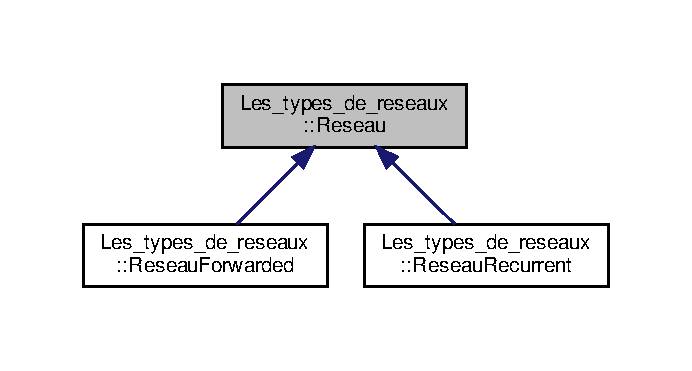
\includegraphics[width=332pt]{class_les__types__de__reseaux_1_1_reseau__inherit__graph}
\end{center}
\end{figure}
\subsection*{Protected Member Functions}
\begin{DoxyCompactItemize}
\item 
\hyperlink{class_les__types__de__reseaux_1_1_reseau_a793f474e4990cfef96ff6af55d146b96}{Reseau} ()
\begin{DoxyCompactList}\small\item\em Constructeurs. \end{DoxyCompactList}\item 
\hyperlink{class_les__types__de__reseaux_1_1_reseau_a519ad4b3e43d46c5840a9d5196fda003}{Reseau} (const int nbC)
\item 
\hyperlink{class_les__types__de__reseaux_1_1_reseau_ac0ff95d39205854ba7bde14d2edba454}{$\sim$\+Reseau} ()
\begin{DoxyCompactList}\small\item\em Destructeur de Couche. \end{DoxyCompactList}\item 
void \hyperlink{class_les__types__de__reseaux_1_1_reseau_ab254177ffab90f08faa97d7810182049}{ajouter\+Couche} (Couche c, int num\+Couche)
\begin{DoxyCompactList}\small\item\em La fonction qui ajoute une couche au réseau Méthode permettant d\textquotesingle{}ajouter autant de couches que l\textquotesingle{}on veut ou qu\textquotesingle{}il est mentionné dans le programme. \end{DoxyCompactList}\item 
void \hyperlink{class_les__types__de__reseaux_1_1_reseau_a71a35e986b54506ca243f3ccb7984fe5}{Apprentissage\+Non\+Supervisé} (Fichier Données)
\begin{DoxyCompactList}\small\item\em La fonction dirige le réseau vers un apprentissage non supervisé en prenant en argument les données fournis en entrée. \end{DoxyCompactList}\end{DoxyCompactItemize}
\subsection*{Protected Attributes}
\begin{DoxyCompactItemize}
\item 
Couche \hyperlink{class_les__types__de__reseaux_1_1_reseau_a5f2f8b87a174fbb7f8f886815adc8728}{Couches} \mbox{[}$\,$\mbox{]}
\item 
int \hyperlink{class_les__types__de__reseaux_1_1_reseau_a990bd80e6670c5bf756aab07ec1a6be4}{nb\+Couche}
\item 
double \hyperlink{class_les__types__de__reseaux_1_1_reseau_a8bbb482e67d52743d91d99912a8ad373}{Matrice\+Liaisons} \mbox{[}$\,$\mbox{]}\mbox{[}$\,$\mbox{]}
\end{DoxyCompactItemize}


\subsection{Detailed Description}
Classe représentant un réseau. 

classe permettant de représenter un réseau quelconque

classe permettant de représenter un réseau quelconque La classe génère le réseau souhaité

Elle permet de générer un réseau

La classe génère le réseau souhaité 

\subsection{Constructor \& Destructor Documentation}
\mbox{\Hypertarget{class_les__types__de__reseaux_1_1_reseau_a793f474e4990cfef96ff6af55d146b96}\label{class_les__types__de__reseaux_1_1_reseau_a793f474e4990cfef96ff6af55d146b96}} 
\index{Les\+\_\+types\+\_\+de\+\_\+reseaux\+::\+Reseau@{Les\+\_\+types\+\_\+de\+\_\+reseaux\+::\+Reseau}!Reseau@{Reseau}}
\index{Reseau@{Reseau}!Les\+\_\+types\+\_\+de\+\_\+reseaux\+::\+Reseau@{Les\+\_\+types\+\_\+de\+\_\+reseaux\+::\+Reseau}}
\subsubsection{\texorpdfstring{Reseau()}{Reseau()}\hspace{0.1cm}{\footnotesize\ttfamily [1/2]}}
{\footnotesize\ttfamily Les\+\_\+types\+\_\+de\+\_\+reseaux\+::\+Reseau\+::\+Reseau (\begin{DoxyParamCaption}{ }\end{DoxyParamCaption})\hspace{0.3cm}{\ttfamily [protected]}}



Constructeurs. 

Constructeurs de la classe Couche


\begin{DoxyParams}{Parameters}
{\em } & \\
\hline
\end{DoxyParams}
\mbox{\Hypertarget{class_les__types__de__reseaux_1_1_reseau_a519ad4b3e43d46c5840a9d5196fda003}\label{class_les__types__de__reseaux_1_1_reseau_a519ad4b3e43d46c5840a9d5196fda003}} 
\index{Les\+\_\+types\+\_\+de\+\_\+reseaux\+::\+Reseau@{Les\+\_\+types\+\_\+de\+\_\+reseaux\+::\+Reseau}!Reseau@{Reseau}}
\index{Reseau@{Reseau}!Les\+\_\+types\+\_\+de\+\_\+reseaux\+::\+Reseau@{Les\+\_\+types\+\_\+de\+\_\+reseaux\+::\+Reseau}}
\subsubsection{\texorpdfstring{Reseau()}{Reseau()}\hspace{0.1cm}{\footnotesize\ttfamily [2/2]}}
{\footnotesize\ttfamily Les\+\_\+types\+\_\+de\+\_\+reseaux\+::\+Reseau\+::\+Reseau (\begin{DoxyParamCaption}\item[{const int}]{nbC }\end{DoxyParamCaption})\hspace{0.3cm}{\ttfamily [protected]}}


\begin{DoxyParams}{Parameters}
{\em nbC} & \+: le nombre de couches qui est fixe d\textquotesingle{}où le \char`\"{}const\char`\"{}Constructeur pour le cas où l\textquotesingle{}utilisateur décide du nombre de couches \\
\hline
\end{DoxyParams}
\mbox{\Hypertarget{class_les__types__de__reseaux_1_1_reseau_ac0ff95d39205854ba7bde14d2edba454}\label{class_les__types__de__reseaux_1_1_reseau_ac0ff95d39205854ba7bde14d2edba454}} 
\index{Les\+\_\+types\+\_\+de\+\_\+reseaux\+::\+Reseau@{Les\+\_\+types\+\_\+de\+\_\+reseaux\+::\+Reseau}!````~Reseau@{$\sim$\+Reseau}}
\index{````~Reseau@{$\sim$\+Reseau}!Les\+\_\+types\+\_\+de\+\_\+reseaux\+::\+Reseau@{Les\+\_\+types\+\_\+de\+\_\+reseaux\+::\+Reseau}}
\subsubsection{\texorpdfstring{$\sim$\+Reseau()}{~Reseau()}}
{\footnotesize\ttfamily Les\+\_\+types\+\_\+de\+\_\+reseaux\+::\+Reseau\+::$\sim$\+Reseau (\begin{DoxyParamCaption}{ }\end{DoxyParamCaption})\hspace{0.3cm}{\ttfamily [protected]}}



Destructeur de Couche. 



\subsection{Member Function Documentation}
\mbox{\Hypertarget{class_les__types__de__reseaux_1_1_reseau_ab254177ffab90f08faa97d7810182049}\label{class_les__types__de__reseaux_1_1_reseau_ab254177ffab90f08faa97d7810182049}} 
\index{Les\+\_\+types\+\_\+de\+\_\+reseaux\+::\+Reseau@{Les\+\_\+types\+\_\+de\+\_\+reseaux\+::\+Reseau}!ajouter\+Couche@{ajouter\+Couche}}
\index{ajouter\+Couche@{ajouter\+Couche}!Les\+\_\+types\+\_\+de\+\_\+reseaux\+::\+Reseau@{Les\+\_\+types\+\_\+de\+\_\+reseaux\+::\+Reseau}}
\subsubsection{\texorpdfstring{ajouter\+Couche()}{ajouterCouche()}}
{\footnotesize\ttfamily Les\+\_\+types\+\_\+de\+\_\+reseaux\+::\+Reseau\+::ajouter\+Couche (\begin{DoxyParamCaption}\item[{Couche}]{c,  }\item[{int}]{num\+Couche }\end{DoxyParamCaption})\hspace{0.3cm}{\ttfamily [protected]}}



La fonction qui ajoute une couche au réseau Méthode permettant d\textquotesingle{}ajouter autant de couches que l\textquotesingle{}on veut ou qu\textquotesingle{}il est mentionné dans le programme. 

\mbox{\Hypertarget{class_les__types__de__reseaux_1_1_reseau_a71a35e986b54506ca243f3ccb7984fe5}\label{class_les__types__de__reseaux_1_1_reseau_a71a35e986b54506ca243f3ccb7984fe5}} 
\index{Les\+\_\+types\+\_\+de\+\_\+reseaux\+::\+Reseau@{Les\+\_\+types\+\_\+de\+\_\+reseaux\+::\+Reseau}!Apprentissage\+Non\+Supervisé@{Apprentissage\+Non\+Supervisé}}
\index{Apprentissage\+Non\+Supervisé@{Apprentissage\+Non\+Supervisé}!Les\+\_\+types\+\_\+de\+\_\+reseaux\+::\+Reseau@{Les\+\_\+types\+\_\+de\+\_\+reseaux\+::\+Reseau}}
\subsubsection{\texorpdfstring{Apprentissage\+Non\+Supervisé()}{ApprentissageNonSupervisé()}}
{\footnotesize\ttfamily Les\+\_\+types\+\_\+de\+\_\+reseaux\+::\+Reseau\+::\+Apprentissage\+Non\+Supervisé (\begin{DoxyParamCaption}\item[{Fichier}]{Données }\end{DoxyParamCaption})\hspace{0.3cm}{\ttfamily [protected]}}



La fonction dirige le réseau vers un apprentissage non supervisé en prenant en argument les données fournis en entrée. 

Méthode permettant d\textquotesingle{}obtenir un réseau pour l\textquotesingle{}apprentissage non supervisé à partir d\textquotesingle{}un fichier donné

\begin{DoxyReturn}{Returns}
Rien mais modifie le réseau 
\end{DoxyReturn}


\subsection{Member Data Documentation}
\mbox{\Hypertarget{class_les__types__de__reseaux_1_1_reseau_a5f2f8b87a174fbb7f8f886815adc8728}\label{class_les__types__de__reseaux_1_1_reseau_a5f2f8b87a174fbb7f8f886815adc8728}} 
\index{Les\+\_\+types\+\_\+de\+\_\+reseaux\+::\+Reseau@{Les\+\_\+types\+\_\+de\+\_\+reseaux\+::\+Reseau}!Couches@{Couches}}
\index{Couches@{Couches}!Les\+\_\+types\+\_\+de\+\_\+reseaux\+::\+Reseau@{Les\+\_\+types\+\_\+de\+\_\+reseaux\+::\+Reseau}}
\subsubsection{\texorpdfstring{Couches}{Couches}}
{\footnotesize\ttfamily Couche Les\+\_\+types\+\_\+de\+\_\+reseaux\+::\+Reseau\+::\+Couches\mbox{[}$\,$\mbox{]}\hspace{0.3cm}{\ttfamily [protected]}}

$<$ Pour que les classes filles aient également accès à ces attributs \mbox{\Hypertarget{class_les__types__de__reseaux_1_1_reseau_a8bbb482e67d52743d91d99912a8ad373}\label{class_les__types__de__reseaux_1_1_reseau_a8bbb482e67d52743d91d99912a8ad373}} 
\index{Les\+\_\+types\+\_\+de\+\_\+reseaux\+::\+Reseau@{Les\+\_\+types\+\_\+de\+\_\+reseaux\+::\+Reseau}!Matrice\+Liaisons@{Matrice\+Liaisons}}
\index{Matrice\+Liaisons@{Matrice\+Liaisons}!Les\+\_\+types\+\_\+de\+\_\+reseaux\+::\+Reseau@{Les\+\_\+types\+\_\+de\+\_\+reseaux\+::\+Reseau}}
\subsubsection{\texorpdfstring{Matrice\+Liaisons}{MatriceLiaisons}}
{\footnotesize\ttfamily double Les\+\_\+types\+\_\+de\+\_\+reseaux\+::\+Reseau\+::\+Matrice\+Liaisons\mbox{[}$\,$\mbox{]}\mbox{[}$\,$\mbox{]}\hspace{0.3cm}{\ttfamily [protected]}}

\mbox{\Hypertarget{class_les__types__de__reseaux_1_1_reseau_a990bd80e6670c5bf756aab07ec1a6be4}\label{class_les__types__de__reseaux_1_1_reseau_a990bd80e6670c5bf756aab07ec1a6be4}} 
\index{Les\+\_\+types\+\_\+de\+\_\+reseaux\+::\+Reseau@{Les\+\_\+types\+\_\+de\+\_\+reseaux\+::\+Reseau}!nb\+Couche@{nb\+Couche}}
\index{nb\+Couche@{nb\+Couche}!Les\+\_\+types\+\_\+de\+\_\+reseaux\+::\+Reseau@{Les\+\_\+types\+\_\+de\+\_\+reseaux\+::\+Reseau}}
\subsubsection{\texorpdfstring{nb\+Couche}{nbCouche}}
{\footnotesize\ttfamily int Les\+\_\+types\+\_\+de\+\_\+reseaux\+::\+Reseau\+::nb\+Couche\hspace{0.3cm}{\ttfamily [protected]}}



The documentation for this class was generated from the following file\+:\begin{DoxyCompactItemize}
\item 
\hyperlink{_reseau_8hpp}{Reseau.\+hpp}\end{DoxyCompactItemize}

\hypertarget{class_les__types__de__reseaux_1_1_reseau_forwarded}{}\doxysection{Les\+\_\+types\+\_\+de\+\_\+reseaux\+::Reseau\+Forwarded Class Reference}
\label{class_les__types__de__reseaux_1_1_reseau_forwarded}\index{Les\_types\_de\_reseaux::ReseauForwarded@{Les\_types\_de\_reseaux::ReseauForwarded}}


Classe permettant de représenter un réseau forwarded.  




{\ttfamily \#include $<$Reseau\+Forwarded.\+hpp$>$}

Inheritance diagram for Les\+\_\+types\+\_\+de\+\_\+reseaux\+::Reseau\+Forwarded\+:\begin{figure}[H]
\begin{center}
\leavevmode
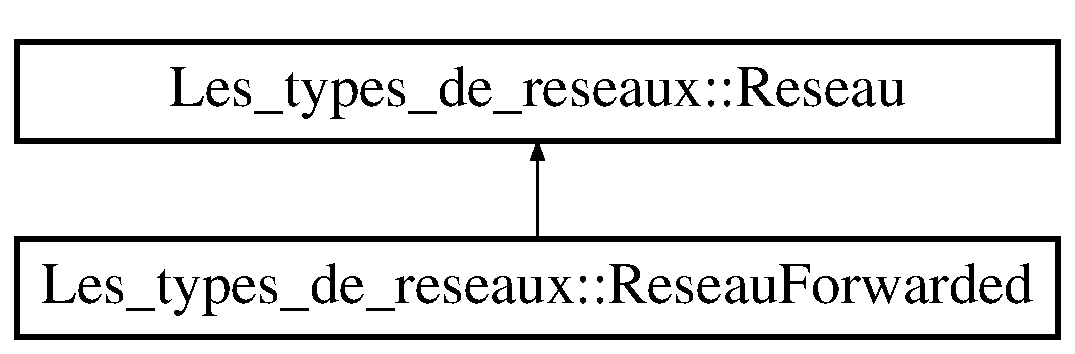
\includegraphics[height=2.000000cm]{class_les__types__de__reseaux_1_1_reseau_forwarded}
\end{center}
\end{figure}
\doxysubsection*{Public Member Functions}
\begin{DoxyCompactItemize}
\item 
\mbox{\hyperlink{class_les__types__de__reseaux_1_1_reseau_forwarded_aebce929c314e9dbfcce8e234cb132083}{Reseau\+Forwarded}} ()
\end{DoxyCompactItemize}
\doxysubsection*{Additional Inherited Members}


\doxysubsection{Detailed Description}
Classe permettant de représenter un réseau forwarded. 

Definition at line 20 of file Reseau\+Forwarded.\+hpp.



\doxysubsection{Constructor \& Destructor Documentation}
\mbox{\Hypertarget{class_les__types__de__reseaux_1_1_reseau_forwarded_aebce929c314e9dbfcce8e234cb132083}\label{class_les__types__de__reseaux_1_1_reseau_forwarded_aebce929c314e9dbfcce8e234cb132083}} 
\index{Les\_types\_de\_reseaux::ReseauForwarded@{Les\_types\_de\_reseaux::ReseauForwarded}!ReseauForwarded@{ReseauForwarded}}
\index{ReseauForwarded@{ReseauForwarded}!Les\_types\_de\_reseaux::ReseauForwarded@{Les\_types\_de\_reseaux::ReseauForwarded}}
\doxysubsubsection{\texorpdfstring{ReseauForwarded()}{ReseauForwarded()}}
{\footnotesize\ttfamily Les\+\_\+types\+\_\+de\+\_\+reseaux\+::\+Reseau\+Forwarded\+::\+Reseau\+Forwarded (\begin{DoxyParamCaption}{ }\end{DoxyParamCaption})}



The documentation for this class was generated from the following file\+:\begin{DoxyCompactItemize}
\item 
\mbox{\hyperlink{_reseau_forwarded_8hpp}{Reseau\+Forwarded.\+hpp}}\end{DoxyCompactItemize}

\hypertarget{class_les__types__de__reseaux_1_1_reseau_recurrent}{}\section{Les\+\_\+types\+\_\+de\+\_\+reseaux\+:\+:Reseau\+Recurrent Class Reference}
\label{class_les__types__de__reseaux_1_1_reseau_recurrent}\index{Les\+\_\+types\+\_\+de\+\_\+reseaux\+::\+Reseau\+Recurrent@{Les\+\_\+types\+\_\+de\+\_\+reseaux\+::\+Reseau\+Recurrent}}


{\ttfamily \#include $<$Reseau\+Recurrent.\+hpp$>$}



Inheritance diagram for Les\+\_\+types\+\_\+de\+\_\+reseaux\+:\+:Reseau\+Recurrent\+:\nopagebreak
\begin{figure}[H]
\begin{center}
\leavevmode
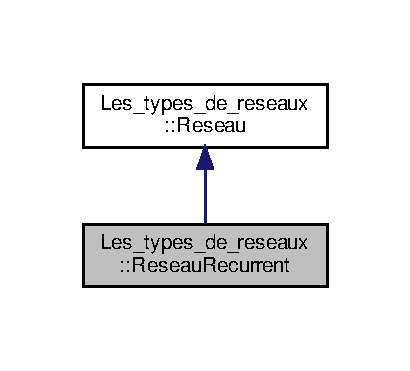
\includegraphics[width=197pt]{class_les__types__de__reseaux_1_1_reseau_recurrent__inherit__graph}
\end{center}
\end{figure}


Collaboration diagram for Les\+\_\+types\+\_\+de\+\_\+reseaux\+:\+:Reseau\+Recurrent\+:\nopagebreak
\begin{figure}[H]
\begin{center}
\leavevmode
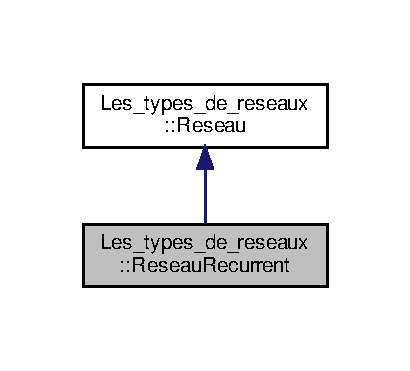
\includegraphics[width=197pt]{class_les__types__de__reseaux_1_1_reseau_recurrent__coll__graph}
\end{center}
\end{figure}
\subsection*{Public Member Functions}
\begin{DoxyCompactItemize}
\item 
\hyperlink{class_les__types__de__reseaux_1_1_reseau_recurrent_a8c63bfcee7b0e29ec1499327366861d6}{Reseau\+Recurrent} ()
\end{DoxyCompactItemize}
\subsection*{Additional Inherited Members}


\subsection{Constructor \& Destructor Documentation}
\mbox{\Hypertarget{class_les__types__de__reseaux_1_1_reseau_recurrent_a8c63bfcee7b0e29ec1499327366861d6}\label{class_les__types__de__reseaux_1_1_reseau_recurrent_a8c63bfcee7b0e29ec1499327366861d6}} 
\index{Les\+\_\+types\+\_\+de\+\_\+reseaux\+::\+Reseau\+Recurrent@{Les\+\_\+types\+\_\+de\+\_\+reseaux\+::\+Reseau\+Recurrent}!Reseau\+Recurrent@{Reseau\+Recurrent}}
\index{Reseau\+Recurrent@{Reseau\+Recurrent}!Les\+\_\+types\+\_\+de\+\_\+reseaux\+::\+Reseau\+Recurrent@{Les\+\_\+types\+\_\+de\+\_\+reseaux\+::\+Reseau\+Recurrent}}
\subsubsection{\texorpdfstring{Reseau\+Recurrent()}{ReseauRecurrent()}}
{\footnotesize\ttfamily Les\+\_\+types\+\_\+de\+\_\+reseaux\+::\+Reseau\+Recurrent\+::\+Reseau\+Recurrent (\begin{DoxyParamCaption}{ }\end{DoxyParamCaption})}



The documentation for this class was generated from the following file\+:\begin{DoxyCompactItemize}
\item 
\hyperlink{_reseau_recurrent_8hpp}{Reseau\+Recurrent.\+hpp}\end{DoxyCompactItemize}

\chapter{File Documentation}
\hypertarget{_couche_8hpp}{}\section{Couche.\+hpp File Reference}
\label{_couche_8hpp}\index{Couche.\+hpp@{Couche.\+hpp}}


\hyperlink{namespace_les}{Les} propriétés d\textquotesingle{}une couche \+: son nombre de neurones ainsi que sa fonction d\textquotesingle{}activation.  


{\ttfamily \#include \char`\"{}Neurone.\+hpp\char`\"{}}\newline
Include dependency graph for Couche.\+hpp\+:\nopagebreak
\begin{figure}[H]
\begin{center}
\leavevmode
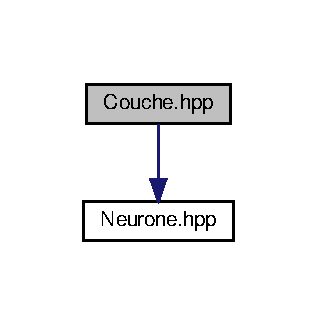
\includegraphics[width=152pt]{_couche_8hpp__incl}
\end{center}
\end{figure}
This graph shows which files directly or indirectly include this file\+:\nopagebreak
\begin{figure}[H]
\begin{center}
\leavevmode
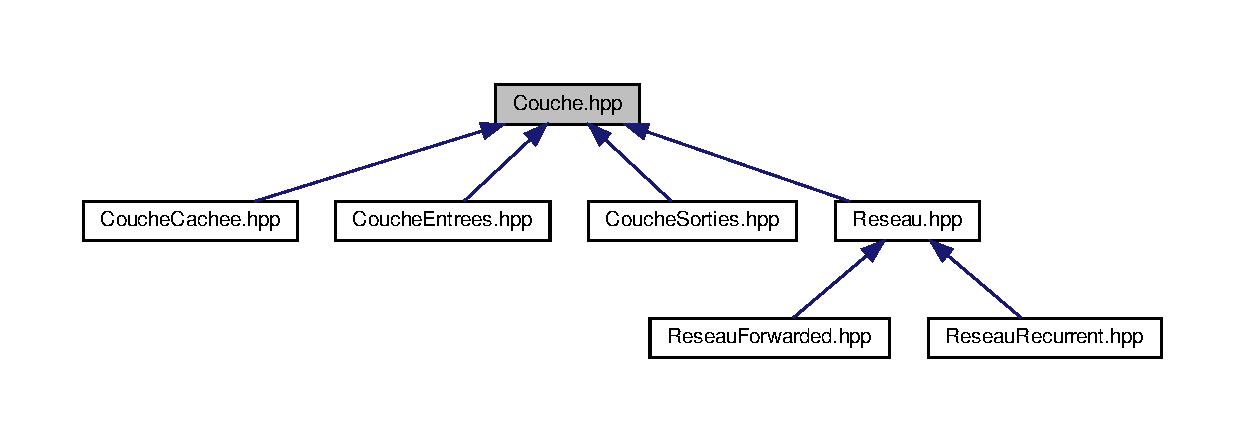
\includegraphics[width=350pt]{_couche_8hpp__dep__incl}
\end{center}
\end{figure}
\subsection*{Classes}
\begin{DoxyCompactItemize}
\item 
class \hyperlink{class_les__couches__du__reseau_1_1_couche}{Les\+\_\+couches\+\_\+du\+\_\+reseau\+::\+Couche}
\begin{DoxyCompactList}\small\item\em Classe représentant une couche. \end{DoxyCompactList}\end{DoxyCompactItemize}
\subsection*{Namespaces}
\begin{DoxyCompactItemize}
\item 
 \hyperlink{namespace_les}{Les}
\item 
 \hyperlink{namespace_les__couches__du__reseau}{Les\+\_\+couches\+\_\+du\+\_\+reseau}
\end{DoxyCompactItemize}


\subsection{Detailed Description}
\hyperlink{namespace_les}{Les} propriétés d\textquotesingle{}une couche \+: son nombre de neurones ainsi que sa fonction d\textquotesingle{}activation. 

\begin{DoxyAuthor}{Author}
Groupe projet A1 
\end{DoxyAuthor}
\begin{DoxyVersion}{Version}
0.\+1 
\end{DoxyVersion}

\hypertarget{_couche_cachee_8hpp}{}\doxysection{/home/camille/\+Bureau/\+G\+M4/\+C++/\+Projet\+\_\+\+C\+P\+P/troisième rendu/\+Couche\+Cachee.hpp File Reference}
\label{_couche_cachee_8hpp}\index{/home/camille/Bureau/GM4/C++/Projet\_CPP/troisième rendu/CoucheCachee.hpp@{/home/camille/Bureau/GM4/C++/Projet\_CPP/troisième rendu/CoucheCachee.hpp}}


C\textquotesingle{}est un classe qui permet de créer les couches cachées du réseau, ainsi que de définir leur biais.  


{\ttfamily \#include \char`\"{}Couche.\+hpp\char`\"{}}\newline
Include dependency graph for Couche\+Cachee.\+hpp\+:
% FIG 0
\doxysubsection*{Classes}
\begin{DoxyCompactItemize}
\item 
class \mbox{\hyperlink{class_les__couches__du__r_xC3_xA9seau_1_1_couche_cachee}{Les\+\_\+couches\+\_\+du\+\_\+réseau\+::\+Couche\+Cachee}}
\end{DoxyCompactItemize}
\doxysubsection*{Namespaces}
\begin{DoxyCompactItemize}
\item 
 \mbox{\hyperlink{namespace_les__couches__du__r_xC3_xA9seau}{Les\+\_\+couches\+\_\+du\+\_\+réseau}}
\end{DoxyCompactItemize}


\doxysubsection{Detailed Description}
C\textquotesingle{}est un classe qui permet de créer les couches cachées du réseau, ainsi que de définir leur biais. 

\begin{DoxyAuthor}{Author}
Groupe projet A1 
\end{DoxyAuthor}
\begin{DoxyVersion}{Version}
0.\+1 
\end{DoxyVersion}

\hypertarget{_couche_entrees_8hpp}{}\doxysection{Couche\+Entrees.\+hpp File Reference}
\label{_couche_entrees_8hpp}\index{CoucheEntrees.hpp@{CoucheEntrees.hpp}}


la couche entrée permet de convertir nos données et d\textquotesingle{}initialiser les entrées de notre réseau  


{\ttfamily \#include \char`\"{}Couche.\+hpp\char`\"{}}\newline
\doxysubsection*{Classes}
\begin{DoxyCompactItemize}
\item 
class \mbox{\hyperlink{class_les__couches__du__reseau_1_1_couche_entrees}{Les\+\_\+couches\+\_\+du\+\_\+reseau\+::\+Couche\+Entrees}}
\begin{DoxyCompactList}\small\item\em Classe représentant la couche d\textquotesingle{}entrée. \end{DoxyCompactList}\end{DoxyCompactItemize}
\doxysubsection*{Namespaces}
\begin{DoxyCompactItemize}
\item 
 \mbox{\hyperlink{namespace_les__couches__du__reseau}{Les\+\_\+couches\+\_\+du\+\_\+reseau}}
\end{DoxyCompactItemize}


\doxysubsection{Detailed Description}
la couche entrée permet de convertir nos données et d\textquotesingle{}initialiser les entrées de notre réseau 

\begin{DoxyAuthor}{Author}
Groupe projet A1 
\end{DoxyAuthor}
\begin{DoxyVersion}{Version}
0.\+1 
\end{DoxyVersion}

\hypertarget{_couche_sorties_8hpp}{}\doxysection{Couche\+Sorties.\+hpp File Reference}
\label{_couche_sorties_8hpp}\index{CoucheSorties.hpp@{CoucheSorties.hpp}}


C\textquotesingle{}est un classe qui permet de créer la couche de sorties du réseau, ainsi que de définir leur biais.  


{\ttfamily \#include \char`\"{}Couche.\+hpp\char`\"{}}\newline
Include dependency graph for Couche\+Sorties.\+hpp\+:
% FIG 0
\doxysubsection*{Classes}
\begin{DoxyCompactItemize}
\item 
class \mbox{\hyperlink{class_les__couches__du__r_xC3_xA9seau_1_1_couche_sorties}{Les\+\_\+couches\+\_\+du\+\_\+réseau\+::\+Couche\+Sorties}}
\end{DoxyCompactItemize}
\doxysubsection*{Namespaces}
\begin{DoxyCompactItemize}
\item 
 \mbox{\hyperlink{namespace_les__couches__du__r_xC3_xA9seau}{Les\+\_\+couches\+\_\+du\+\_\+réseau}}
\end{DoxyCompactItemize}


\doxysubsection{Detailed Description}
C\textquotesingle{}est un classe qui permet de créer la couche de sorties du réseau, ainsi que de définir leur biais. 

\begin{DoxyAuthor}{Author}
Groupe projet A1 
\end{DoxyAuthor}
\begin{DoxyVersion}{Version}
0.\+1 
\end{DoxyVersion}

\hypertarget{_interface_8hpp}{}\section{Interface.\+hpp File Reference}
\label{_interface_8hpp}\index{Interface.\+hpp@{Interface.\+hpp}}


Interface Utilisateur permet de saisir divers paramètres par l\textquotesingle{}utilisateur du réseau.  


\subsection*{Classes}
\begin{DoxyCompactItemize}
\item 
class \hyperlink{class_interface___saisie__des__donnees_1_1_interface}{Interface\+\_\+\+Saisie\+\_\+des\+\_\+donnees\+::\+Interface}
\begin{DoxyCompactList}\small\item\em Classe ou l\textquotesingle{}utilisateur saisit les paramètres, et choix des différentes options proposées pour son futur réseau. \end{DoxyCompactList}\end{DoxyCompactItemize}
\subsection*{Namespaces}
\begin{DoxyCompactItemize}
\item 
 \hyperlink{namespace_interface___saisie__des__donnees}{Interface\+\_\+\+Saisie\+\_\+des\+\_\+donnees}
\end{DoxyCompactItemize}


\subsection{Detailed Description}
Interface Utilisateur permet de saisir divers paramètres par l\textquotesingle{}utilisateur du réseau. 

\begin{DoxyAuthor}{Author}
Groupe projet A1 
\end{DoxyAuthor}
\begin{DoxyVersion}{Version}
0.\+1 
\end{DoxyVersion}

\hypertarget{_matrice_8hpp}{}\section{Matrice.\+hpp File Reference}
\label{_matrice_8hpp}\index{Matrice.\+hpp@{Matrice.\+hpp}}


Une classe qui définit quelques opérations matricielles.  


\subsection*{Classes}
\begin{DoxyCompactItemize}
\item 
class \hyperlink{class_les__types__de__reseaux_1_1_matrice}{Les\+\_\+types\+\_\+de\+\_\+reseaux\+::\+Matrice}
\end{DoxyCompactItemize}
\subsection*{Namespaces}
\begin{DoxyCompactItemize}
\item 
 \hyperlink{namespace_les__types__de__reseaux}{Les\+\_\+types\+\_\+de\+\_\+reseaux}
\end{DoxyCompactItemize}


\subsection{Detailed Description}
Une classe qui définit quelques opérations matricielles. 

\begin{DoxyAuthor}{Author}
Groupe projet A1 
\end{DoxyAuthor}
\begin{DoxyVersion}{Version}
0.\+1 
\end{DoxyVersion}

\hypertarget{_neurone_8hpp}{}\doxysection{Neurone.\+hpp File Reference}
\label{_neurone_8hpp}\index{Neurone.hpp@{Neurone.hpp}}


Les propritées d\textquotesingle{}un neurone \+: son indice et so valeur.  


\doxysubsection*{Classes}
\begin{DoxyCompactItemize}
\item 
class \mbox{\hyperlink{class_les__couches__du__reseau_1_1_neurone}{Les\+\_\+couches\+\_\+du\+\_\+reseau\+::\+Neurone}}
\begin{DoxyCompactList}\small\item\em Classe représentant un neurone. \end{DoxyCompactList}\end{DoxyCompactItemize}
\doxysubsection*{Namespaces}
\begin{DoxyCompactItemize}
\item 
 \mbox{\hyperlink{namespace_les__couches__du__reseau}{Les\+\_\+couches\+\_\+du\+\_\+reseau}}
\end{DoxyCompactItemize}


\doxysubsection{Detailed Description}
Les propritées d\textquotesingle{}un neurone \+: son indice et so valeur. 

\begin{DoxyAuthor}{Author}
Groupe projet A1 
\end{DoxyAuthor}
\begin{DoxyVersion}{Version}
0.\+1 
\end{DoxyVersion}

\hypertarget{_reseau_8hpp}{}\doxysection{Reseau.\+hpp File Reference}
\label{_reseau_8hpp}\index{Reseau.hpp@{Reseau.hpp}}


Les propriétés d\textquotesingle{}un réseau \+: le nombre de couches qui le compose, ses couches, et sa matrice de liaison.  


{\ttfamily \#include \char`\"{}Couche.\+hpp\char`\"{}}\newline
\doxysubsection*{Classes}
\begin{DoxyCompactItemize}
\item 
class \mbox{\hyperlink{class_les__types__de__reseaux_1_1_reseau}{Les\+\_\+types\+\_\+de\+\_\+reseaux\+::\+Reseau}}
\begin{DoxyCompactList}\small\item\em Classe représentant un réseau. \end{DoxyCompactList}\end{DoxyCompactItemize}
\doxysubsection*{Namespaces}
\begin{DoxyCompactItemize}
\item 
 \mbox{\hyperlink{namespace_les__types__de__reseaux}{Les\+\_\+types\+\_\+de\+\_\+reseaux}}
\end{DoxyCompactItemize}


\doxysubsection{Detailed Description}
Les propriétés d\textquotesingle{}un réseau \+: le nombre de couches qui le compose, ses couches, et sa matrice de liaison. 

\begin{DoxyAuthor}{Author}
Groupe projet A1 
\end{DoxyAuthor}
\begin{DoxyVersion}{Version}
0.\+1 
\end{DoxyVersion}

\hypertarget{_reseau_forwarded_8hpp}{}\doxysection{/home/camille/\+Bureau/\+G\+M4/\+C++/\+Projet\+\_\+\+C\+P\+P/troisième rendu/\+Reseau\+Forwarded.hpp File Reference}
\label{_reseau_forwarded_8hpp}\index{/home/camille/Bureau/GM4/C++/Projet\_CPP/troisième rendu/ReseauForwarded.hpp@{/home/camille/Bureau/GM4/C++/Projet\_CPP/troisième rendu/ReseauForwarded.hpp}}


C\textquotesingle{}est un classe qui permet de spécifier le type de réseau désiré, ici \+: type feed-\/forwarded, permet donc de préciser les arguments (forme du réseau)  


{\ttfamily \#include \char`\"{}Reseau.\+hpp\char`\"{}}\newline
Include dependency graph for Reseau\+Forwarded.\+hpp\+:
% FIG 0
\doxysubsection*{Classes}
\begin{DoxyCompactItemize}
\item 
class \mbox{\hyperlink{class_les__types__de__r_xC3_xA9seaux_1_1_reseau_forwarded}{Les\+\_\+types\+\_\+de\+\_\+réseaux\+::\+Reseau\+Forwarded}}
\end{DoxyCompactItemize}
\doxysubsection*{Namespaces}
\begin{DoxyCompactItemize}
\item 
 \mbox{\hyperlink{namespace_les__types__de__r_xC3_xA9seaux}{Les\+\_\+types\+\_\+de\+\_\+réseaux}}
\end{DoxyCompactItemize}


\doxysubsection{Detailed Description}
C\textquotesingle{}est un classe qui permet de spécifier le type de réseau désiré, ici \+: type feed-\/forwarded, permet donc de préciser les arguments (forme du réseau) 

\begin{DoxyAuthor}{Author}
Groupe projet A1 
\end{DoxyAuthor}
\begin{DoxyVersion}{Version}
0.\+1 
\end{DoxyVersion}

\hypertarget{_reseau_recurrent_8hpp}{}\doxysection{Reseau\+Recurrent.\+hpp File Reference}
\label{_reseau_recurrent_8hpp}\index{ReseauRecurrent.hpp@{ReseauRecurrent.hpp}}


C\textquotesingle{}est un classe qui permet de spécifier le type de réseau désiré, ici \+: type récurrent, permet donc de préciser les arguments (forme du réseau spécifique)  


{\ttfamily \#include \char`\"{}Reseau.\+hpp\char`\"{}}\newline
\doxysubsection*{Classes}
\begin{DoxyCompactItemize}
\item 
class \mbox{\hyperlink{class_les__types__de__reseaux_1_1_reseau_recurrent}{Les\+\_\+types\+\_\+de\+\_\+reseaux\+::\+Reseau\+Recurrent}}
\begin{DoxyCompactList}\small\item\em classe permettant de représenter un réseau récurrent \end{DoxyCompactList}\end{DoxyCompactItemize}
\doxysubsection*{Namespaces}
\begin{DoxyCompactItemize}
\item 
 \mbox{\hyperlink{namespace_les__types__de__reseaux}{Les\+\_\+types\+\_\+de\+\_\+reseaux}}
\end{DoxyCompactItemize}


\doxysubsection{Detailed Description}
C\textquotesingle{}est un classe qui permet de spécifier le type de réseau désiré, ici \+: type récurrent, permet donc de préciser les arguments (forme du réseau spécifique) 

\begin{DoxyAuthor}{Author}
Groupe projet A1 
\end{DoxyAuthor}
\begin{DoxyVersion}{Version}
0.\+1 
\end{DoxyVersion}

%--- End generated contents ---

% Index
\backmatter
\newpage
\phantomsection
\clearemptydoublepage
\addcontentsline{toc}{chapter}{Index}
\printindex

\end{document}
